\documentclass[11pt]{article}

%%%%%%%%%%%%%%%%%%%%%%%%%%%%%%%%%%%%%%%%%%%%%%%%%%%%%%%%%%%%%%%%%%%%%%%%%%%%%%%
% 1. CONFIGURACIÓN DEL DOCUMENTO, IDIOMA Y CODIFICACIÓN
%%%%%%%%%%%%%%%%%%%%%%%%%%%%%%%%%%%%%%%%%%%%%%%%%%%%%%%%%%%%%%%%%%%%%%%%%%%%%%%

% --- Codificación y Geometría ---
% \usepackage[utf8]{inputenc} % (Recomendado si usas pdfLaTeX)
% \usepackage[T1]{fontenc}    % (Recomendado para fuentes y guiones)

\usepackage[spanish,es-tabla]{babel} % Soporte para idioma español, separación silábica y nombres
\usepackage{csquotes}                % Soporte avanzado para comillas y citas (funciona con babel)
\usepackage[a4paper, margin=2cm, marginparwidth=3cm]{geometry} % Configura márgenes y tamaño de página

%%%%%%%%%%%%%%%%%%%%%%%%%%%%%%%%%%%%%%%%%%%%%%%%%%%%%%%%%%%%%%%%%%%%%%%%%%%%%%%
% 2. PAQUETES DE MATEMÁTICA Y FÍSICA
%%%%%%%%%%%%%%%%%%%%%%%%%%%%%%%%%%%%%%%%%%%%%%%%%%%%%%%%%%%%%%%%%%%%%%%%%%%%%%%

\usepackage{amsmath}   % Comandos avanzados para entornos matemáticos
\usepackage{amssymb}   % Símbolos matemáticos extendidos (como \mathbb)
\usepackage{bbold}     % Fuentes "Blackboard" (para números 0, 1)
\usepackage{bigints}   % Símbolos de integrales más grandes
\usepackage{physics}   % Notación común en física (derivadas, \bra, \ket, etc.)
\usepackage{cancel}    % Para tachar expresiones matemáticas
\usepackage{bm}        % Para usar negrita en modo matemática

%%%%%%%%%%%%%%%%%%%%%%%%%%%%%%%%%%%%%%%%%%%%%%%%%%%%%%%%%%%%%%%%%%%%%%%%%%%%%%%
% 3. GRÁFICOS, FIGURAS, COLORES Y DIBUJO (TIKZ)
%%%%%%%%%%%%%%%%%%%%%%%%%%%%%%%%%%%%%%%%%%%%%%%%%%%%%%%%%%%%%%%%%%%%%%%%%%%%%%%

\usepackage[table,xcdraw,x11names]{xcolor}      % Gestión avanzada de colores (usado por TikZ, listings, etc.)
\usepackage{graphicx}                           % Para incluir imágenes (.png, .jpg, .pdf)
\usepackage[export]{adjustbox}                  % Herramientas extra para imágenes (recortar, enmarcar)
\usepackage{float}                              % Mejor control sobre la posición de flotantes [H]
\usepackage[font=small, labelfont=bf]{caption}  % Personalización de los pies de foto/tabla
\usepackage{subcaption}                         % Para crear subfiguras y subtables
\usepackage{tikz}                               % Potente sistema para crear gráficos vectoriales
\usepackage{circuitikz}                         % Extensión de TikZ para dibujar circuitos eléctricos

% --- Librerías y definiciones de TikZ ---
\usetikzlibrary{patterns, decorations.markings, arrows.meta}
\usetikzlibrary{decorations.pathreplacing}
\usetikzlibrary{decorations.pathmorphing}
\definecolor{ForestGreen}{rgb}{0.13, 0.55, 0.13}    % Define un color personalizado
\definecolor{Yellow}{HTML}{91760D}                  % Define un color personalizado


%%%%%%%%%%%%%%%%%%%%%%%%%%%%%%%%%%%%%%%%%%%%%%%%%%%%%%%%%%%%%%%%%%%%%%%%%%%%%%%
% 4. FORMATO DE PÁGINA, SECCIONES Y LISTAS
%%%%%%%%%%%%%%%%%%%%%%%%%%%%%%%%%%%%%%%%%%%%%%%%%%%%%%%%%%%%%%%%%%%%%%%%%%%%%%%

\usepackage{titlesec}     % Personalización avanzada de títulos de sección
\usepackage{multicol}     % Para crear texto en múltiples columnas
\usepackage{enumitem}     % Personalización avanzada de listas (enumerate, itemize)
\usepackage{wrapfig}      % Para que el texto fluya alrededor de una figura
\usepackage{booktabs}     % Crea tablas con aspecto profesional (mejores líneas)
\usepackage{setspace}     % Permite cambiar el interlineado (ej. \onehalfspacing)
\usepackage{yfonts}       % Permite usar fuentes góticas (\textfrak)
\usepackage{fontawesome}  % Íconos de Font Awesome

%%%%%%%%%%%%%%%%%%%%%%%%%%%%%%%%%%%%%%%%%%%%%%%%%%%%%%%%%%%%%%%%%%%%%%%%%%%%%%%
% 5. UTILIDADES Y ENTORNOS ESPECIALES
%%%%%%%%%%%%%%%%%%%%%%%%%%%%%%%%%%%%%%%%%%%%%%%%%%%%%%%%%%%%%%%%%%%%%%%%%%%%%%%

\usepackage{todonotes}          % Añade notas (TODOs) en el margen o en línea
\usepackage[most]{tcolorbox}    % Crea cajas de texto coloreadas y personalizables
\usepackage{listings}           % Para insertar bloques de código fuente (Syntax Highlighting)
\usepackage{pdfpages}           % Para incluir páginas de otros documentos PDF
\usepackage{lipsum}             % Genera texto de relleno (Lorem Ipsum)
\usepackage{bm}

%%%%%%%%%%%%%%%%%%%%%%%%%%%%%%%%%%%%%%%%%%%%%%%%%%%%%%%%%%%%%%%%%%%%%%%%%%%%%%%
% 6. ENCABEZADOS, PIES DE PÁGINA E ÍNDICES (TOC)
%%%%%%%%%%%%%%%%%%%%%%%%%%%%%%%%%%%%%%%%%%%%%%%%%%%%%%%%%%%%%%%%%%%%%%%%%%%%%%%

\usepackage{tocloft}      % Personalización de la Tabla de Contenidos (ToC)
\usepackage{fancyhdr}     % Para personalizar encabezados y pies de página
\usepackage{lastpage}     % Provee una referencia a la última página (para "Pág X de Y")

%%%%%%%%%%%%%%%%%%%%%%%%%%%%%%%%%%%%%%%%%%%%%%%%%%%%%%%%%%%%%%%%%%%%%%%%%%%%%%%
% 7. HIPERVÍNCULOS (IMPORTANTE: Cargar casi al final)
%%%%%%%%%%%%%%%%%%%%%%%%%%%%%%%%%%%%%%%%%%%%%%%%%%%%%%%%%%%%%%%%%%%%%%%%%%%%%%%

% Generalmente es mejor cargar hyperref al final, ya que modifica
% muchos comandos de LaTeX.
\usepackage[colorlinks=true, allcolors=black]{hyperref} 

%%%%%%%%%%%%%%%%%%%%%%%%%%%%%%%%%%%%%%%%%%%%%%%%%%%%%%%%%%%%%%%%%%%%%%%%%%%%%%%
% 8. CONFIGURACIONES Y COMANDOS PERSONALIZADOS
% (Deben ir después de cargar sus paquetes correspondientes)
%%%%%%%%%%%%%%%%%%%%%%%%%%%%%%%%%%%%%%%%%%%%%%%%%%%%%%%%%%%%%%%%%%%%%%%%%%%%%%%

% --- Config. Mates (amsmath) ---
% Numera las ecuaciones como (sección.numero)
\numberwithin{equation}{section} 

% --- Config. Secciones y TOC (titlesec, babel) ---
% Formato para párrafos como si fueran subtítulos
\titleformat{\paragraph}[block]{\normalfont\normalsize\bfseries}{\theparagraph}{1em}{}
\setcounter{secnumdepth}{4} % Profundidad de numeración de secciones
\setcounter{tocdepth}{4}    % Profundidad del índice (TOC)

% --- Config. Encabezados (fancyhdr) ---
\pagestyle{fancy}                                   % Activa el estilo personalizado
\fancyhf{}                                          % Limpia todos los campos de encabezado y pie
\setlength{\headheight}{16pt}                       % Aumenta el espacio para el encabezado
\fancyhead[R]{\rightmark}                           % Pone el nombre de la sección/subsección a la derecha
\cfoot{\thepage \hspace{1pt} de \pageref{LastPage}} % Pie de página centrado "Página X de Y"

% Asegura que las subsecciones actualicen \rightmark (para el encabezado)
\addto\captionsspanish{\renewcommand{\subsectionmark}[1]{\markright{#1}}}

% --- Config. Layout (multicol) ---
\setlength\columnsep{18pt}          % Separación entre columnas

% --- Config. Utilidades (todonotes) ---
\setuptodonotes{inline, size=\footnotesize, color=blue!20, bordercolor=none}

% --- Config. Código (listings) ---
\lstdefinelanguage{custombash}{
    language=bash,
    morekeywords={conda, activate, mkdir, cd, cmake, make, git, sudo},
    sensitive=true
}

\lstdefinestyle{bashStyle}{
    language=custombash,
    basicstyle=\ttfamily\small,
    keywordstyle=\color{teal}\bfseries,
    commentstyle=\color{gray}\itshape,
    stringstyle=\color{orange},
    identifierstyle=\color{black},
    numbers=left,
    numberstyle=\tiny\color{gray},
    stepnumber=1,
    numbersep=10pt,
    backgroundcolor=\color{white},
    showspaces=false,
    showstringspaces=false,
    breaklines=true,
    frame=single,
    captionpos=b
}

\lstdefinestyle{pythonStyle}{
    language=Python,
    basicstyle=\ttfamily\small,
    keywordstyle=\color{blue}\bfseries,
    commentstyle=\color{gray}\itshape,
    stringstyle=\color{orange},
    identifierstyle=\color{black},
    numbers=left,
    numberstyle=\tiny\color{gray},
    stepnumber=1,
    numbersep=10pt,
    backgroundcolor=\color{white},
    showspaces=false,
    showstringspaces=false,
    breaklines=true,
    frame=single,
    captionpos=b
}

\lstdefinestyle{cppStyle}{
    language=C++,
    basicstyle=\ttfamily\small,
    keywordstyle=\color{blue}\bfseries,
    commentstyle=\color{gray}\itshape,
    stringstyle=\color{red},
    numbers=left,
    numberstyle=\tiny\color{gray},
    stepnumber=1,
    numbersep=10pt,
    backgroundcolor=\color{white},
    showspaces=false,
    showstringspaces=false,
    breaklines=true,
    frame=single,
    captionpos=b
}

% --- Comandos Personalizados ---

% Comando para texto en un círculo (requiere TikZ)
\newcommand*\circled[1]{\tikz[baseline=(char.base)]{\node[shape=circle,draw,inner sep=1.5pt] (char) {#1};}}

% Comando para tachar con color (requiere cancel y xcolor)
\newcommand{\colorcancel}[2]{\textcolor{#1}{\cancel{\textcolor{black}{#2}}}}

% --- Entornos Personalizados (tcolorbox) ---
\newtcolorbox{infobox}[2][blue]{
    colback=#1!5!white,
    colframe=#1!75!black,
    title={#2},
    fonttitle=\bfseries,
    coltitle=black,
    boxrule=0.8pt,
    arc=4pt,
    left=6pt,
    right=6pt,
    top=6pt,
    bottom=6pt,
    breakable
}

%%%%%%%%%%%%%%%%%%%%%%%%%%%%%%%%%%%%%%%%%%%%%%%%%%%%%%%%%%%%%%%%%%%%%%%%%%%%%%%

% Comando personalizado para CosmoLattice
\usepackage{xspace}
\newcommand{\CosmoLattice}{\ensuremath{\mathcal{C}}\text{osmo}\ensuremath{\mathcal{L}}\text{attice}\xspace}


% Referencia a una sección que puede estar en otra rama: si la etiqueta existe, "Sec. X";
% si no, "la rama <nombre>".
\newcommand{\reframa}[2]{\ifcsname r@#1\endcsname Sec.~\ref{#1}\else la rama \texttt{#2}\fi}

\begin{document}
    \sloppy

    \section*{Introducción y organización}

        Estudiamos el fondo de ondas gravitacionales (GWs) que produce el \emph{preheating} después de la inflación, simulado en la red con \CosmoLattice, para modelos de inflación cuyo potencial se comporta como $|\phi|^n$ cerca del mínimo: monomiales generalizados $A|\phi|^n$, T-models $A\tanh^n(\phi/M)$ y E-models $A(1-e^{-\phi/M})^n$. El caso de referencia es $n = 4$ con los parámetros que favorecen las observaciones del CMB según Ellis, Garcia, Olive \& Verner (2026) (Sec.~\ref{sec:parametros-cuarticos}). Para $n = 4$ el espectro de hoy no depende de la historia de reheating (Sec.~\ref{sec:reescaleo}). Como comparación corremos también los casos cuadráticos ($n = 2$, Sec.~\ref{sec:parametros-cuadraticos}), cuyo espectro de hoy sí depende de la temperatura de reheating (Sec.~\ref{sec:resultados-cuadraticos}).

        El repositorio está organizado en ramas:
        \begin{itemize}
            \item \texttt{main} tiene lo general. Son estas notas: el marco común (Sec.~\ref{sec:marco}), los parámetros del paper, el análisis y el reescaleo a hoy, los requisitos de cómputo y la guía de uso. También tiene el código de análisis y CosmoLattice.
            \item \texttt{monomial}, \texttt{t-model} y \texttt{e-model} agregan, cada una, el modelo de \CosmoLattice (\texttt{.h}), sus \texttt{.in} y su sección de estas notas, que aparece al final al compilar en esa rama.
        \end{itemize}
        Las referencias a secciones de un modelo que no está en la rama actual aparecen como ``la rama \texttt{...}''.

    \section{Marco común: potenciales con mínimo $|\phi|^n$}
        \label{sec:marco}

        Los tres tipos de modelo se comportan cerca del mínimo como $V \simeq A_{\text{eff}} |\phi|^n$, con $A_{\text{eff}} = A$ (monomial) o $A_{\text{eff}} = A/M^n$ (T y E). Todo lo que depende sólo de ese comportamiento está en esta sección; lo propio de cada potencial (derivadas, $\phi_0$ explícito) está en la sección de cada modelo, en su rama.

        \subsection{Variables de programa}
            \label{sec:variables}

            Cerca del mínimo, la ecuación de movimiento del modo homogéneo del campo es
            \begin{equation}
                \ddot{\phi} + 3 H \dot{\phi} + \Omega^2(\phi) \, \phi = 0 \, ,
                \hspace{1cm}
                \Omega^2(\phi) \equiv \frac{V^\prime(\phi)}{\phi} \simeq n A_{\text{eff}} \, |\phi|^{n-2} \, ,
            \end{equation}
            es decir, un oscilador de frecuencia $\Omega(\phi)$ que depende de la amplitud (excepto para $n=2$). Para que el exponente $\alpha$ de la Sec.~\ref{sec:alpha} cumpla su propósito (período de oscilación aproximadamente constante en tiempo de programa), $\omega_*$ debe ser precisamente esta frecuencia física evaluada en la amplitud inicial $\phi_0$. Usamos la amplitud efectiva local y no la altura global del potencial, porque durante el reheating el campo oscila en $|\phi| \lesssim M$ (prescripción de \CosmoLattice, arXiv:2006.15122, Sec.~8):
            \begin{equation}
                f_* = \phi_0 \, , \hspace{1cm}
                \omega_* \equiv \Omega(\phi_0) = \sqrt{n A_{\text{eff}}} \, \phi_0^{n/2 - 1} \, .
            \end{equation}
            Con el acople $\frac12 g^2\phi^2\chi^2$ y $\tilde V = V/(f_*^2\omega_*^2)$, cerca del mínimo
            \begin{equation}
                \tilde{V} \left( \tilde{\phi}, \tilde{\chi} \right) \simeq \frac{1}{n} \left| \tilde{\phi} \right|^n + \frac{1}{2} \, q \, \tilde{\phi}^2 \tilde{\chi}^2 \, ,
                \hspace{1cm}
                q \equiv \frac{g^2 \phi_0^2}{\omega_*^2} = \frac{g^2 \phi_0^{4-n}}{n A_{\text{eff}}} \, .
            \end{equation}
            El factor $1/n$ es el de la normalización estándar de \CosmoLattice (\texttt{lphi4} escribe $V = \frac{\lambda}{4} \phi^4$, es decir $A = \lambda/4$); con $n=4$ y $A=\lambda/4$ se recupera $\omega_* = \sqrt{\lambda}\,\phi_0$, como en \texttt{lphi4.h}. Para $n = 4$, $\omega_*/f_* = \sqrt{4A_{\text{eff}}} \equiv \sqrt{\lambda_{\text{eff}}}$ no depende de $\phi_0$.

        \subsection{Reescaleo temporal}
            \label{sec:alpha}

            Además de $f_*$ y $\omega_*$, \CosmoLattice permite elegir un exponente de reescaleo temporal $\alpha$, definido a través de $d\tilde{t} = \omega_* a^{-\alpha} dt$. Con $\omega_* = \Omega(\phi_0)$ fijado como arriba, $\alpha$ debe elegirse de forma que $\Omega(\phi)$ siga siendo aproximadamente constante en tiempo de programa a lo largo de \emph{toda} la fase de oscilaciones post-inflacionarias, no sólo en $\phi = \phi_0$.

            Para un potencial monomial $V \sim |\phi|^n$, la solución autosimilar de las oscilaciones post-inflacionarias del campo homogéneo (ver p.ej.\ Turner 1983, y la discusión en la Sec.~8 de Figueroa, Florio, Torrenti \& Valkenburg, arXiv:2006.15122) da una frecuencia de oscilación que decae con la expansión como $\Omega \sim a^{-3(n-2)/(n+2)}$. Pidiendo que esa frecuencia sea constante en tiempo de programa se obtiene
            \begin{equation}
                \alpha = 3 \, \frac{n - 2}{n + 2}
            \end{equation}
            Esta fórmula es consistente con los modelos ya implementados en \CosmoLattice: \texttt{lphi4} ($n=4$) usa $\alpha = 1$, y \texttt{tanh2} ($n=2$) usa $\alpha = 0$, ambos reproducidos por la expresión anterior. La misma elección vale para los T-models y E-models, que se reducen a un monomial de índice $n$ cerca de $\phi = 0$, la región que domina la dinámica durante el reheating.

        \subsection{Condiciones iniciales: $\epsilon_V = 1$}
            \label{sec:ci}

            Tomamos como condición inicial el punto en que termina el slow-roll según el parámetro del potencial,
            \begin{equation}
                \epsilon_V(\phi_0) = \frac{m_p^2}{2} \left[ \frac{V^\prime (\phi_0)}{V(\phi_0)} \right]^2 = 1 \, ,
            \end{equation}
            que es lo que usa \texttt{tanh2.in}. La solución explícita para $\phi_0$ depende del potencial y está en la sección de cada modelo: $\phi_0 = n m_p/\sqrt 2$ (monomial), $\phi_0 = \frac{M}{2}\operatorname{arcsinh}(\sqrt2 n m_p/M)$ (T) y $\phi_0 = M\ln(1 + n m_p/(\sqrt 2 M))$ (E).

        \subsection{Momento inicial}
            \label{sec:momento-inicial}

            En $\epsilon = 1$ el campo ya está rodando, así que el momento inicial no puede ser nulo (\texttt{tanh2.in} usa, por ejemplo, $\dot\phi_0 = -3.07 \times 10^{31}\,\text{GeV}^2$). Tomamos la velocidad de slow-roll, pero con el $H$ autoconsistente, que incluye la energía cinética:
            \begin{equation}
                \dot{\phi} = -\frac{V^\prime}{3H} \, ,
                \hspace{1cm}
                H^2 = \frac{1}{3 m_p^2} \left( V + \frac{1}{2} \dot{\phi}^2 \right) \, .
            \end{equation}
            Elevando al cuadrado la primera y reemplazando la segunda queda una cuadrática en $\dot\phi^2$:
            \begin{equation*}
                \begin{split}
                    9 H^2 \dot{\phi}^2 &= V^{\prime 2}\\
                    \frac{3}{m_p^2} \left( V + \frac{1}{2} \dot{\phi}^2 \right) \dot{\phi}^2 &= V^{\prime 2}\\
                    \frac{3}{2} \dot{\phi}^4 + 3 V \dot{\phi}^2 - m_p^2 V^{\prime 2} &= 0\\
                    \dot{\phi}^2 &= -V + \sqrt{V^2 + \frac{2}{3} m_p^2 V^{\prime 2}} \, .
                \end{split}
            \end{equation*}
            En $\phi_0$, la condición $\epsilon = 1$ es justamente $m_p^2 V^{\prime 2} = 2 V^2$, de modo que
            \begin{equation}
                \dot{\phi}_0 = - \sqrt{ \left( \sqrt{\tfrac{7}{3}} - 1 \right) V(\phi_0) } \simeq -0.726 \, \sqrt{V(\phi_0)} \, ,
            \end{equation}
            con el signo negativo porque $\phi_0 > 0$ y el campo rueda hacia el mínimo. El resultado sólo usa $\epsilon = 1$, así que vale igual para los T-models y los E-models, cambiando únicamente $V(\phi_0)$. Con los parámetros de \texttt{tanh2.in} esta fórmula da $-3.02 \times 10^{31}\,\text{GeV}^2$, un $2\%$ por debajo del valor de \CosmoLattice.

            Nótese que $\epsilon = 1$ es la condición de slow-roll ($\epsilon_V$), no el final exacto de la inflación ($\epsilon_H \equiv -\dot H/H^2 = \frac{3}{2}\dot\phi^2/\rho = 1$): con el momento de arriba, $\epsilon_H(\phi_0) \simeq 0.63$. Cuánto se aparta $\epsilon_V = 1$ del final exacto, integrando el fondo homogéneo, está en la sección de cada modelo. Usamos $\epsilon_V = 1$ por consistencia con \texttt{tanh2.in}. Los números los recalcula \texttt{code/verificar\_genmodels.py}.

        \subsection{Estabilidad numérica para $n > 4$}
            \label{sec:estabilidad}

            En variables de programa, la ecuación de movimiento de \CosmoLattice para cada campo es (arXiv:2006.15122)
            \begin{equation}
                \tilde{\phi}^{\prime\prime} + (3 - \alpha) \frac{a^\prime}{a} \tilde{\phi}^\prime - a^{-2(1-\alpha)} \tilde{\nabla}^2 \tilde{\phi} + a^{2\alpha} \frac{\partial \tilde{V}}{\partial \tilde{\phi}} = 0 \, ,
            \end{equation}
            de modo que un modo de número de onda $\tilde k$ oscila con frecuencia
            \begin{equation}
                \tilde{\omega}_{\tilde k}^2 = a^{2\alpha - 2} \tilde{k}^2 + a^{2\alpha} \, \frac{\partial^2 \tilde{V}}{\partial \tilde{\phi}^2} \, .
            \end{equation}
            El integrador (\texttt{VV2}, tipo leapfrog) es estable sólo si $\tilde{\omega}_{\max} \, \delta\tilde{t} < 2$. Con la amplitud de las oscilaciones autosimilares, $\tilde{\Phi} \propto a^{-6/(n+2)}$, y $\alpha = 3(n-2)/(n+2)$, cada término escala así:
            \begin{itemize}
                \item \textbf{Inflatón:} $a^{2\alpha} (n-1) \tilde\Phi^{n-2} \propto a^{0}$. Es constante, porque $\alpha$ se eligió precisamente para eso.
                \item \textbf{Gradiente:} $a^{\alpha-1} \tilde{k}_{\max} \propto a^{2(n-4)/(n+2)}$, con $\tilde{k}_{\max} = 2\sqrt{3}/\delta\tilde{x}$ y $\delta\tilde x = 2\pi / (N \tilde{k}_{\text{IR}})$ para el laplaciano de segundo orden.
                \item \textbf{Campo hijo:} $a^{\alpha} \sqrt{q} \, \tilde\Phi \propto \sqrt{q} \, a^{3(n-4)/(n+2)}$.
            \end{itemize}
            Para $n \le 4$ ningún término crece (en $n = 4$, \texttt{lphi4}, son constantes). Para $n > 4$ los dos últimos crecen sin cota, de modo que con $\delta\tilde t$ fijo la simulación se vuelve inestable a partir de
            \begin{equation}
                a_{\max}^{\text{grad}} = \left( \frac{2}{\tilde{k}_{\max} \, \delta\tilde{t}} \right)^{\frac{n+2}{2(n-4)}} \, ,
                \hspace{1cm}
                a_{\max}^{\text{hijo}} \sim \left( \frac{2}{\sqrt{q} \, \delta\tilde{t}} \right)^{\frac{n+2}{3(n-4)}} \, .
            \end{equation}
            La segunda es sólo una estimación, porque toma la envolvente de $\tilde\phi$ normalizada a $1$ en $a = 1$ y no tiene en cuenta el crecimiento resonante de $\chi$. Esto no se arregla con otra elección de $\alpha$: físicamente, para $n > 4$ la frecuencia del inflatón decae más rápido que $k/a$ y que la masa efectiva $g \Phi$ del campo hijo, así que la separación entre escalas crece con cualquier reescaleo temporal. Lo mismo vale para los T-models y E-models con $n > 4$, que cerca de $\phi = 0$ son monomiales.
            Un ejemplo con $n = 6$, comparado con una corrida, está en \reframa{sec:monomial}{monomial}.

    \section{Parámetros cosmológicos para modelos cuárticos ($n = 4$)}
        \label{sec:parametros-cuarticos}

        \subsection{Traducción desde Ellis, Garcia, Olive \& Verner}

            Ellis, Garcia, Olive \& Verner, \emph{Phys.\ Rev.\ D} \textbf{113}, 063571 (2026) [doi:10.1103/d35r-7bn8], contrastan los $\alpha$-attractors generalizados con Planck 2018, BICEP/Keck, ACT DR6 y SPT-3G. Sus potenciales (Ecs.~39--40) son
            \begin{equation}
                V_E = \frac{3}{4} \lambda m_p^4 \left( 1 - e^{-\sqrt{\frac{2}{3\alpha_K}} \frac{\phi}{m_p}} \right)^k \, ,
                \hspace{1cm}
                V_T = \frac{3}{4} \lambda m_p^4 \tanh^k \left( \frac{\phi}{\sqrt{6 \alpha_K} \, m_p} \right) \, ,
            \end{equation}
            donde llamamos $\alpha_K$ al $\alpha$ del potencial de Kähler, para no confundirlo con el exponente de reescaleo temporal $\alpha$ de \CosmoLattice (que para $n = 4$ vale $\alpha = 1$). En nuestra notación ($V = A |f(\phi/M)|^n$) esto es
            \begin{equation}
                n = k \, , \hspace{1cm}
                A = \frac{3}{4} \lambda m_p^4 \, , \hspace{1cm}
                M_E = \sqrt{\tfrac{3}{2} \alpha_K} \, m_p \, , \hspace{1cm}
                M_T = \sqrt{6 \alpha_K} \, m_p \, .
            \end{equation}

        \subsection{Por qué $k = 4$ y qué valores elegir}

            Para $k = 4$ la ecuación de estado del inflatón oscilando es $w = (k-2)/(k+2) = 1/3$, y el término de reheating de $N_*$ se anula (Sec.~VII.B del paper): $N_* \simeq 55.7$ (E) y $55.8$ (T) para $\alpha_K = 1$, independientemente de $T_{\text{RH}}$ (Ec.~B15). Por eso $n_s$ y $r$ dependen sólo de $\alpha_K$ y, para las ondas gravitacionales, el universo se expande como radiación desde el final de la inflación, de modo que el corrimiento al rojo del espectro hasta hoy no depende de la historia de reheating. Además, por la Sec.~\ref{sec:estabilidad}, $n = 4$ no tiene la inestabilidad creciente de $n > 4$.

            Lo que el paper encuentra para $k = 4$:
            \begin{itemize}
                \item \textbf{E-model:} $\alpha_K = 1$ da $n_s \simeq 0.965$, que atraviesa las elipses de Planck 2018 y es compatible con CMB-SPA; con $\alpha_K \simeq 5$ entra apenas en el $95\%$ de P-ACT-LB. La cota en $r$ da $\alpha_K \lesssim 17$.
                \item \textbf{T-model:} $\alpha_K \lesssim 11$ es compatible con Planck 2018 y con el $95\%$ de CMB-SPA, aunque queda por debajo de ACT DR6.
            \end{itemize}
            Elegimos como casos de referencia el canónico $\alpha_K = 1$ para ambos modelos, y $\alpha_K = 5$ en el E-model como el más cercano a ACT. En vez de la Ec.~38 del paper ($\lambda \simeq 24 \alpha_K \pi^2 A_s / N_*^2$, aproximada) normalizamos $\lambda$ exactamente con $A_s = V/(24\pi^2 \epsilon_V m_p^4) = 2.1 \times 10^{-9}$ en $\phi_*$. Para eso calculamos $\phi_{\text{end}}$ ($\epsilon_H = 1$, fondo exacto) y $\phi_*$ ($N_*$ e-folds antes, Ec.~18). Las condiciones iniciales son las de la Sec.~\ref{sec:ci} ($\epsilon_V = 1$), con las fórmulas de cada modelo (\reframa{sec:tmodel}{t-model} y \reframa{sec:emodel}{e-model}).

            \begin{table}[H]
                \centering
                \begin{tabular}{lccc}
                    \toprule
                    & E, $\alpha_K = 1$ & T, $\alpha_K = 1$ & E, $\alpha_K = 5$ \\
                    \midrule
                    $N_*$ & $55.7$ & $55.8$ & $55.7$ \\
                    $n_s$ & $0.9647$ & $0.9641$ & $0.9652$ \\
                    $r$ & $0.0036$ & $0.0038$ & $0.0153$ \\
                    $\lambda$ & $1.528 \times 10^{-10}$ & $1.600 \times 10^{-10}$ & $7.12 \times 10^{-10}$ \\
                    $H_*$ [GeV] & $1.49 \times 10^{13}$ & $1.52 \times 10^{13}$ & $3.06 \times 10^{13}$ \\
                    \midrule
                    \texttt{n} & $4$ & $4$ & $4$ \\
                    \texttt{M} [GeV] & $2.98225 \times 10^{18}$ & $5.96451 \times 10^{18}$ & $6.66852 \times 10^{18}$ \\
                    \texttt{A} [GeV$^4$] & $4.02858 \times 10^{63}$ & $4.21854 \times 10^{63}$ & $1.87750 \times 10^{64}$ \\
                    \texttt{initial\_amplitudes} [GeV] & $3.56906 \times 10^{18}$ & $4.69413 \times 10^{18}$ & $4.73073 \times 10^{18}$ \\
                    \texttt{initial\_momenta} [GeV$^2$] & $-2.2449 \times 10^{31}$ & $-2.0345 \times 10^{31}$ & $-2.5689 \times 10^{31}$ \\
                    $\omega_*$ [GeV] & $5.09 \times 10^{13}$ & $1.71 \times 10^{13}$ & $2.92 \times 10^{13}$ \\
                    $\lambda_{\text{eff}} = 4A/M^4$ & $2.04 \times 10^{-10}$ & $1.33 \times 10^{-11}$ & $3.80 \times 10^{-11}$ \\
                    \bottomrule
                \end{tabular}
                \caption{Casos de referencia para $n = 4$ y valores para \texttt{genemodel.in} / \texttt{gentmodel.in} ($m_p = 2.435 \times 10^{18}$\,GeV). Los recalcula \texttt{code/parametros\_cuarticos.py}.}
                \label{tab:parametros-cuarticos}
            \end{table}

            Como chequeo, el mismo código con $\alpha_K = 1$ y $N_* = 55$ reproduce la Tabla~II del paper: $n_s = 0.9643$ (E) y $0.9636$ (T), idénticos, y $r$ a menos del $1\%$ (el paper calcula las perturbaciones exactas; nosotros usamos slow-roll). La Ec.~38 del paper sobreestima $\lambda$ en un $5\%$ (E, $\alpha_K = 1$) y un $13\%$ (E, $\alpha_K = 5$); para el T-model coincide.

            Dos observaciones. Primero, $\phi_0/M = 1.20$ (E, $\alpha_K = 1$), $0.79$ (T) y $0.71$ (E, $\alpha_K = 5$): al principio el campo no está en la región cuártica, y $\omega_*$ (calculado con la aproximación local $A/M^n$) es sólo una escala de referencia hasta que la amplitud cae por debajo de $M$. Segundo, el paper no fija el acople $g$, de modo que $q$ sigue siendo una elección nuestra. Cerca del mínimo el potencial de programa es $\tilde\phi^4/4 + \tfrac12 q \tilde\phi^2\tilde\chi^2$, igual que en \texttt{lphi4}, con $q = g^2/\lambda_{\text{eff}}$; un punto de partida razonable es el $q = 300$ de \texttt{lphi4.in}.

    \section{Parámetros cosmológicos para modelos cuadráticos ($n = 2$)}
        \label{sec:parametros-cuadraticos}

        \subsection{El número de e-folds depende de $T_{\text{RH}}$}

            Para $k = 2$ (el T-model y el E-model canónicos, que con $\alpha_K = 1$ es Starobinsky) el inflatón oscila como materia, $w = 0$, hasta que decae. Entonces el último término de la Ec.~27 del paper no se anula, como pasaba para $k = 4$, y $N_*$ depende de la temperatura de reheating. Con $w_{\text{int}} = 0$,
            \begin{equation}
                N_* = 61.49 - \frac{1}{12}\ln g_{\text{RH}} + \frac14 \ln\frac{V_*^2}{m_p^4\,\rho_{\text{end}}} + \frac{1}{12}\ln\frac{\rho_{\text{RH}}}{\rho_{\text{end}}} \, ,
                \hspace{1cm}
                \rho_{\text{RH}} = \frac{\pi^2}{30} g_{\text{RH}} T_{\text{RH}}^4 \, ,
            \end{equation}
            con $g_{\text{RH}} = 915/4$ (MSSM, como el paper) y $\rho_{\text{end}}$ la densidad en $\epsilon_H = 1$, del fondo exacto. Como $\lambda$, y con ella $V_*$ y $\rho_{\text{end}}$, depende de $\phi_*$, la ecuación se resuelve en forma autoconsistente (\texttt{code/parametros\_cuadraticos.py}). Como chequeo, con $\alpha_K = 1$ el resultado queda $0.15$--$0.17$ e-folds por debajo de las aproximaciones analíticas B9 (E) y B10 (T) del paper, que según el mismo paper tienen un error de hasta $0.2\%$. Además reproduce su ejemplo de la Sec.~VII.A: $N_* = 50$ para $T_{\text{RH}} \simeq 5 \times 10^7$\,GeV, con $n_s = 0.961$.

        \subsection{Qué valores elegir}

            Según el paper (Sec.~VII.A y Fig.~2), con $\alpha_K = 1$ los dos modelos son compatibles con el límite inferior de $n_s$ de Planck 2018 (al $95\%$) para $220\,\text{GeV} \lesssim T_{\text{RH}} \lesssim 10^{10}$\,GeV (E) y $2 \times 10^4\,\text{GeV} \lesssim T_{\text{RH}} \lesssim 10^{10}$\,GeV (T). Ninguno entra en el $95\%$ de P-ACT-LB para ningún $T_{\text{RH}}$. Valores mayores de $\alpha_K$ reducen la tensión (la cota en $r$ da $\alpha_K \lesssim 25$ para E y $\lesssim 11$ para T). Elegimos:
            \begin{itemize}
                \item los mismos $\alpha_K$ que en el caso cuártico, para poder comparar: E y T con $\alpha_K = 1$, y E con $\alpha_K = 5$;
                \item $T_{\text{RH}} = 10^{10}$\,GeV: es la cota de gravitinos, cae dentro de la ventana de Planck para los dos modelos y es la que da el $n_s$ más alto de esa ventana (el más cercano a ACT).
            \end{itemize}
            Ese $T_{\text{RH}}$ también entra en el reescaleo a hoy de las GWs (Sec.~\ref{sec:reescaleo}).

            \begin{table}[H]
                \centering
                \begin{tabular}{lcccc}
                    \toprule
                    & E, $\alpha_K = 1$ & T, $\alpha_K = 1$ & E, $\alpha_K = 5$ & $\phi^2$ (control) \\
                    \midrule
                    $N_*$ & $51.6$ & $51.8$ & $52.1$ & $51.8$ \\
                    $n_s$ & $0.9626$ & $0.9615$ & $0.9645$ & $0.9617$ \\
                    $r$ & $0.0040$ & $0.0043$ & $0.0151$ & $0.153$ \\
                    $\lambda$ & $1.691 \times 10^{-10}$ & $1.843 \times 10^{-10}$ & $7.01 \times 10^{-10}$ & -- \\
                    $H_*$ [GeV] & $1.56 \times 10^{13}$ & $1.63 \times 10^{13}$ & $3.04 \times 10^{13}$ & -- \\
                    \midrule
                    \texttt{M} [GeV] & $2.98225 \times 10^{18}$ & $5.96451 \times 10^{18}$ & $6.66852 \times 10^{18}$ & -- \\
                    \texttt{A} & $4.45852 \times 10^{63}$ & $4.85975 \times 10^{63}$ & $1.84811 \times 10^{64}$ & $1.36605 \times 10^{26}$ \\
                    \texttt{initial\_amplitudes} [GeV] & $2.28933 \times 10^{18}$ & $2.94243 \times 10^{18}$ & $2.77636 \times 10^{18}$ & $3.44361 \times 10^{18}$ \\
                    \texttt{initial\_momenta} [GeV$^2$] & $-2.5990 \times 10^{31}$ & $-2.3131 \times 10^{31}$ & $-3.3625 \times 10^{31}$ & $-2.9233 \times 10^{31}$ \\
                    $\omega_* = m$ [GeV] & $3.17 \times 10^{13}$ & $1.65 \times 10^{13}$ & $2.88 \times 10^{13}$ & $1.65 \times 10^{13}$ \\
                    $\phi_0/M$ & $0.77$ & $0.49$ & $0.42$ & -- \\
                    \bottomrule
                \end{tabular}
                \caption{Casos cuadráticos con $T_{\text{RH}} = 10^{10}$\,GeV. \texttt{A} está en GeV$^4$ en los T/E-models y en GeV$^2$ en el monomial ($V = A\phi^2$). $n_s$ y $r$ son de slow-roll (el paper da los exactos). Los recalcula \texttt{code/parametros\_cuadraticos.py}.}
                \label{tab:parametros-cuadraticos}
            \end{table}

            Para $n = 2$, $\omega_* = \sqrt{2A}/M$ es la masa del inflatón en el mínimo, $\alpha = 0$ (el tiempo de programa es $\tilde t = m t$) y el potencial de programa cerca del mínimo es $\tilde\phi^2/2 + \tfrac12 q\tilde\phi^2\tilde\chi^2$, con $q = g^2\phi_0^2/m^2$. La masa del E-model con $\alpha_K = 1$, $3.2 \times 10^{13}$\,GeV, es la conocida de Starobinsky. El monomial de control, $V = m^2\phi^2/2$, usa la masa del T-model con $\alpha_K = 1$, así que tiene el mismo potencial cerca del mínimo; está excluido por $r$. Arranca en $\phi_0 = \sqrt 2\, m_p$ ($\epsilon_V = 1$).

            El paper no fija el acople $g$. Usamos $q = 4 \times 10^4$, el de \texttt{tanh2.in} de \CosmoLattice, en los cuatro casos. Con ese $q$ la resonancia es ancha y las GWs salen en $\tilde k \sim 50$.

    \section{Análisis de las corridas y reescaleo a hoy}
        \label{sec:analisis}

        El script \texttt{code/analisis\_cosmolattice.py} lee el directorio de salida de una corrida y produce seis gráficos (fondo, campos, espectros de los campos, errores, GWs y energías) más un \texttt{resumen.txt}. Las fórmulas de esta sección están verificadas con sympy en \texttt{code/verificar\_reescaleo.py}, y el reescaleo a hoy está implementado en \texttt{code/reescaleo\_gws.py}.

        \subsection{Qué escribe \CosmoLattice}

            Todo está en variables de programa: $\tilde t$ con $d\tilde t = \omega_* a^{-\alpha} dt$, $\tilde k = k/\omega_*$, $\tilde\phi = \phi/f_*$ y $\tilde\rho = \rho/(f_*^2\omega_*^2)$, con $a = 1$ al comienzo. El script lee los parámetros del \texttt{<modelo>.infos} que deja la corrida y recalcula $f_*$, $\omega_*$ y $\alpha$ con las fórmulas de la Sec.~\ref{sec:variables} (o las de \texttt{lphi4}). Los archivos que usa son:
            \begin{itemize}
                \item \texttt{average\_scale\_factor.txt}: $\tilde t$, $a$, $a' = da/d\tilde t$ y $a'/a$. El Hubble físico es $H = \omega_* a^{-\alpha} \, a'/a$.
                \item \texttt{average\_scalar\_i.txt}: $\langle\tilde\phi\rangle$, $\langle\tilde\phi'\rangle$, sus cuadrados y sus rms.
                \item \texttt{average\_energies.txt}: $\tilde\rho$ cinético y de gradiente de cada campo, cada término del potencial y el total.
                \item \texttt{average\_energy\_conservation.txt}: el error relativo de la primera ecuación de Friedmann.
                \item \texttt{spectra\_scalar\_i.txt}: un bloque por tiempo (los tiempos están en \texttt{average\_spectra\_times.txt}) con $\tilde k$, $\Delta_{\tilde\phi}(\tilde k)$, $\Delta_{\tilde\phi'}(\tilde k)$ y la multiplicidad del bin.
                \item \texttt{spectra\_energy\_gws.txt} y \texttt{average\_energies\_gws.txt}: $\Omega_{GW}(\tilde k, \tilde t) = \rho_{\text{tot}}^{-1} \, d\rho_{GW}/d\log k$ (normalizado por la densidad total, no por la crítica, aunque con expansión autoconsistente son lo mismo; nota técnica~II de \CosmoLattice, Sec.~4), y la integral $\rho_{GW}/\rho_{\text{tot}}$.
            \end{itemize}

        \subsection{Fondo y dinámica de los campos}

            La presión se arma con los términos de energía: para cada escalar $\tilde p = \tilde K - \tilde G/3 - \tilde V$ (para campos gauge, $\tilde p = \tilde\rho/3$), y $w = \tilde p / \tilde\rho$. Para un condensado que oscila en $V \propto |\phi|^n$, el teorema del virial da $\langle\dot\phi^2\rangle = n\langle V\rangle$, y entonces
            \begin{equation}
                \langle w \rangle = \frac{n-2}{n+2} \, , \hspace{1cm}
                \rho \propto a^{-3(1+w)} = a^{-6n/(n+2)} \, , \hspace{1cm}
                \Phi \propto a^{-6/(n+2)} \, ,
            \end{equation}
            donde $\Phi$ es la amplitud de las oscilaciones. El script grafica $w$ instantáneo y promediado, $\tilde\rho \, a^{3(1+w_n)}$ (constante si el fondo es autosimilar) y $a^{6/(n+2)}\langle\tilde\phi\rangle$ (oscilación de amplitud constante mientras el condensado domina). Para $n = 4$: $w = 1/3$ y $\Phi \propto a^{-1}$. El promedio de $w$ se toma sobre períodos enteros de $\langle\tilde\phi\rangle$, medidos de sus cruces por cero, porque el período en $\tilde t$ depende de la amplitud: en \texttt{lphi4} es $T \simeq 6.52$ y no el $7.42$ de amplitud unidad.

        \subsection{Chequeos de errores}

            En variables de programa (verificado con sympy partiendo de las ecuaciones en tiempo cósmico):
            \begin{align}
                a'^2 &= \frac{a^{2\alpha+2}}{3} \left( \frac{f_*}{m_p} \right)^2 \tilde\rho \, , \label{eq:friedmann1}\\
                a'' &= \frac{a^{2\alpha+1}}{6} \left( \frac{f_*}{m_p} \right)^2 \left[ (2\alpha - 1) \tilde\rho - 3\tilde p \right] \, , \label{eq:friedmann2}\\
                \tilde\rho' &= -3 \frac{a'}{a} \left( \tilde\rho + \tilde p \right) \, , \label{eq:continuidad}
            \end{align}
            y la Ec.~\eqref{eq:continuidad} no depende de $\alpha$. Como chequeo, con $\alpha = 1$ y radiación ($\tilde p = \tilde\rho/3$) la Ec.~\eqref{eq:friedmann2} da $a'' = 0$, es decir $a \propto \tilde t$ (tiempo conforme). El script grafica:
            \begin{itemize}
                \item el error de la Ec.~\eqref{eq:friedmann1}, que calcula \CosmoLattice;
                \item los residuos de \eqref{eq:friedmann2} y \eqref{eq:continuidad}, con las derivadas calculadas por un spline cúbico de la salida. Estos residuos están limitados por \texttt{tOutputFreq}: con diferencias centradas daban $\sim 2\%$, y con el spline quedan en $\sim 4 \times 10^{-4}$, del orden del error de Friedmann;
                \item la cola UV, $\Delta(\tilde k_{\max})/\max\Delta$, de cada espectro: si no es chica, falta resolución;
                \item la integral $\sum \Omega_{GW} \, \Delta k/k$ contra el $\rho_{GW}/\rho$ que escribe \CosmoLattice;
                \item $aH/k_{\text{IR}}$, que tiene que ser $< 1$. Si no, hay modos de GWs fuera del horizonte, que no se diluyen como radiación y para los que el reescaleo de abajo no vale.
            \end{itemize}

        \subsection{Reescaleo a hoy}
            \label{sec:reescaleo}

            Sea $a_e$ el factor de escala al final de la simulación (con $a_i = 1$) y $\rho_e$ la densidad total en ese momento. Suponemos que entre $a_e$ y el comienzo de la dominación por radiación $a_{RD}$ la ecuación de estado es la autosimilar, $w = (n-2)/(n+2)$, y que después se conserva la entropía. Entonces
            \begin{equation}
                \rho_{RD} = \rho_e \left( \frac{a_e}{a_{RD}} \right)^{3(1+w)} = \frac{\pi^2}{30} g_* T_{RD}^4 \, ,
                \hspace{1cm}
                \frac{a_{RD}}{a_0} = \left( \frac{g_{s0}}{g_{s*}} \right)^{1/3} \frac{T_0}{T_{RD}} \, .
            \end{equation}
            Combinándolas (y usando $a_e/a_{RD} = (\rho_{RD}/\rho_e)^{1/4} \epsilon^{1/4}$),
            \begin{equation}
                \frac{a_e}{a_0} = \frac{\epsilon^{1/4}}{\rho_e^{1/4}} \, T_0 \left( \frac{\pi^2 g_*}{30} \right)^{1/4} \left( \frac{g_{s0}}{g_{s*}} \right)^{1/3} \, ,
                \hspace{1cm}
                \epsilon \equiv \left( \frac{a_e}{a_{RD}} \right)^{1 - 3w} = \left( \frac{a_e}{a_{RD}} \right)^{\frac{2(4-n)}{n+2}} \, .
            \end{equation}
            \paragraph{Frecuencia.} Un modo comóvil $k$ tiene hoy $f_0 = k/(2\pi a_0)$. Escribiendo $k = \tilde k \, \omega_*$ y $\rho_e = \tilde\rho_e f_*^2 \omega_*^2$,
            \begin{equation}
                \boxed{
                f_0 = \frac{\tilde k}{a_e \, \tilde\rho_e^{1/4}} \left( \frac{\omega_*}{f_*} \right)^{1/2} \epsilon^{1/4} \; C_f \, ,
                \hspace{1cm}
                C_f = \frac{T_0}{2\pi} \left( \frac{\pi^2 g_*}{30} \right)^{1/4} \left( \frac{g_{s0}}{g_{s*}} \right)^{1/3} = 4.59 \times 10^{10}\,\text{Hz}
                }
            \end{equation}
            para el Modelo Estándar ($g_* = g_{s*} = 106.75$, $g_{s0} = 3.909$, $T_0 = 2.7255$\,K). La dependencia en el modelo entra por $\omega_*/f_*$ y por $n$ (a través de $\epsilon$):
            \begin{equation}
                \frac{\omega_*}{f_*} = \sqrt{nA} \, \phi_0^{\frac{n-4}{2}} \;\; \text{(monomial)} \, ,
                \hspace{1cm}
                \frac{\omega_*}{f_*} = \sqrt{nA} \, M^{-n/2} \, \phi_0^{\frac{n-4}{2}} \;\; \text{(T y E)} \, .
            \end{equation}
            Para $n = 4$ no dependen de $\phi_0$: $\omega_*/f_* = \sqrt{4A}/M^2 = \sqrt{\lambda_{\text{eff}}}$ (T/E) y $\sqrt{\lambda}$ en \texttt{lphi4}.
            \paragraph{Amplitud.} Las GWs se diluyen como radiación, $\rho_{GW} \propto a^{-4}$, así que $\Omega_{GW,0} = \Omega_{GW,e} \, \rho_e (a_e/a_0)^4 / \rho_{c,0}$. Escribiendo $\rho_{c,0} = \rho_{\gamma,0}/\Omega_{\gamma,0}$ con $\rho_{\gamma,0} = (\pi^2/30) \, 2 \, T_0^4$,
            \begin{equation}
                \boxed{
                h^2 \Omega_{GW,0}(f_0) = C_\Omega \; \epsilon \; \Omega_{GW,e}(\tilde k) \, ,
                \hspace{1cm}
                C_\Omega = h^2 \Omega_{\gamma,0} \, \frac{g_*}{2} \left( \frac{g_{s0}}{g_{s*}} \right)^{4/3} = 1.61 \times 10^{-5}
                }
            \end{equation}
            con $h^2\Omega_{\gamma,0} = 2.474 \times 10^{-5}$. La amplitud no depende de $\omega_*$: sólo de $n$, a través de $\epsilon$.
            \paragraph{El caso cuártico.} Para $n = 4$ se tiene $1 - 3w = 0$, y entonces $\epsilon = 1$ exactamente, sin importar cuándo empieza la dominación por radiación: el resultado no depende de la historia de reheating, igual que el $N_*$ de la Sec.~\ref{sec:parametros-cuarticos}. Así,
            \begin{equation}
                f_0 = \frac{\tilde k \sqrt{\lambda_{\text{eff}}}}{a_e \, \tilde\rho_e^{1/4}} \times 4.59 \times 10^{10}\,\text{Hz} \, ,
                \hspace{1cm}
                h^2\Omega_{GW,0} = 1.61 \times 10^{-5} \; \Omega_{GW,e} \, .
            \end{equation}
            Para $n \ne 4$ hay que dar $a_e/a_{RD}$ (opción \texttt{--a\_e\_sobre\_a\_RD}). Si el inflatón se fragmenta, $w \to 1/3$ antes y $\epsilon \to 1$ (Sec.~VII.B de Ellis \emph{et al.}).
            \paragraph{El caso cuadrático.} Para $n = 2$, $w = 0$ y $\epsilon = a_e/a_{RD}$. Si el universo se comporta como materia desde el final de la simulación hasta el reheating, $a_e/a_{RD} = (\rho_{RD}/\rho_e)^{1/3}$, con $\rho_{RD} = (\pi^2 g_*/30)\,T_{\text{RH}}^4$. Entonces
            \begin{equation}
                h^2\Omega_{GW,0} \propto \epsilon = \left(\frac{\rho_{RD}}{\rho_e}\right)^{1/3} \, ,
                \hspace{1cm}
                f_0 \propto \epsilon^{1/4} \, ,
            \end{equation}
            y la señal se diluye tanto más cuanto más bajo es $T_{\text{RH}}$. El analizador lo calcula con \texttt{--TRH} (y con \texttt{--w\_post} se puede usar otra ecuación de estado entre $a_e$ y $a_{RD}$). Es el mismo factor que dan Dufaux \emph{et al.}\ (arXiv:0707.0875, nota al pie~4 de la Sec.~III.D y Sec.~VIII) para una etapa intermedia de materia que va de $a_1$ a $a_2$: la amplitud baja en $a_1/a_2$ y la frecuencia en $(a_1/a_2)^{1/4}$. Esta suposición es la más pesimista: en las corridas, al final de la simulación $\langle w\rangle \simeq 0.25$--$0.29$, no $0$, porque buena parte de la energía está en fluctuaciones semirrelativistas de los dos campos (Sec.~\ref{sec:resultados-cuadraticos}, «Por qué $\langle w\rangle$ no es 0»). Por eso damos también la cota opuesta, $\epsilon = 1$ (radiación desde el final de la simulación). Con $T_{\text{RH}} = 10^{10}$\,GeV los dos casos difieren en unos cinco órdenes de magnitud en la amplitud (Sec.~\ref{sec:resultados-cuadraticos}).

        \subsection{Comparación con la literatura}
            \label{sec:literatura}

            \begin{itemize}
                \item \textbf{Dufaux \emph{et al.}\ 2007} (arXiv:0707.0875, Ecs.~45--47) escriben $f = k/(a_j\rho_j^{1/4}) \times 4 \times 10^{10}$\,Hz y $\Omega_{gw}h^2 = \Omega_{\text{rad}}h^2 (g_*/g_0)^{-1/3} \, \epsilon \, \Omega_{GW,e}$, con $g_*/g_0 = 100$, $g = g_s$ y $\Omega_{\text{rad}}h^2 = 4.3 \times 10^{-5}$ (lo que da $9.3 \times 10^{-6}$). Nuestras fórmulas se reducen exactamente a las suyas con $g_s = g$ (verificado con sympy). Con sus mismas hipótesis dan $C_f = 3.97 \times 10^{10}$\,Hz, y $C_\Omega = 9.26 \times 10^{-6}$ si se usa su $\Omega_{\text{rad}}h^2$ (con el nuestro, $4.16 \times 10^{-5}$, da $8.96 \times 10^{-6}$).
                \item \textbf{Figueroa \& Torrentí 2017} (arXiv:1707.04533, Ecs.~2.24--2.27) usan la misma cadena de factores de escala y el mismo $\epsilon = (a/a_{RD})^{1-3w}$. Para la amplitud, $h^2\Omega_{\text{rad}}(g_o/g_{RD})^{1/3}$ coincide con nuestro $C_\Omega$ salvo un factor $(g_{s0}/g_0)^{4/3} = 1.22$, porque ellos toman $g_s = g$ también hoy. Para la frecuencia escriben $8 \times 10^9$\,Hz, mientras que su propia expresión con $\rho_o = 2 \times 10^{-15}\,\text{eV}^4$ da $\rho_o^{1/4}/(2\pi) = 5.1 \times 10^{10}$\,Hz, un factor $6.4 \approx 2\pi$ mayor. No pudimos reconciliar ese factor a partir del texto; nuestro $C_f$ coincide con el de Dufaux \emph{et al.}
                \item \textbf{Prueba de punta a punta}: corrimos \texttt{lphi4} con los parámetros de Dufaux \emph{et al.}\ ($q = g^2/\lambda = 120$, hasta $\tilde t = 240$; $N = 64$, $\tilde k_{\text{IR}} = 0.7$, \texttt{withGWs = true}) y la analizamos con el script. El fondo sigue a la radiación: $\langle w\rangle = 0.334$ en los dos últimos períodos. El error de Friedmann queda por debajo de $4.0 \times 10^{-4}$, y $k_{\text{IR}}/(aH) = 162$ al final, así que todos los modos de GWs están dentro del horizonte. El pico final da $h^2\Omega_{GW,0} = 7.0 \times 10^{-11}$ en $f_0 = 1.09 \times 10^8$\,Hz, contra $h^2\Omega_{gw} \sim 3 \times 10^{-11}$ en $f \sim 7 \times 10^7$\,Hz del paper (su Fig.~4). Pasado a sus constantes ($9.3 \times 10^{-6}$ y $4 \times 10^{10}$\,Hz) nuestro pico queda en $4.1 \times 10^{-11}$ y $9.5 \times 10^7$\,Hz: un factor $\sim 1.4$ en ambos. Es una concordancia razonable, porque el espectro es ancho (varía menos de un factor 2 en $1 \lesssim \tilde k \lesssim 10$), nuestra caja es chica ($\Delta \tilde k / \tilde k = 20\%$ en el pico) y el código y las condiciones iniciales son distintos. No es una reproducción fina.
            \end{itemize}

        \subsection{Uso}

            {\footnotesize\begin{verbatim}
python3 code/analisis_cosmolattice.py DIR_DE_LA_CORRIDA [--gstar 106.75] [--a_e_sobre_a_RD 1]
python3 code/verificar_reescaleo.py      # sympy + comparación con la literatura
            \end{verbatim}}
            Para que haya espectro de GWs hay que correr con \texttt{withGWs = true}.

    \section{Corridas cuárticas: archivos y requisitos de memoria y tiempo}
        \label{sec:recursos}

        \subsection{Los \texttt{.in}}
            \label{sec:in}

            Los tres casos de la Tabla~\ref{tab:parametros-cuarticos} quedaron en \texttt{models/parameter-files/}: \texttt{gentmodel\_cuartico.in} (T, $\alpha_K = 1$), \texttt{genemodel\_cuartico.in} (E, $\alpha_K = 1$) y \texttt{genemodel\_cuartico\_aK5.in} (E, $\alpha_K = 5$); el monomial de control \texttt{genmonomial\_cuartico.in} se describe en \reframa{sec:control}{monomial}. Los tres usan \texttt{withGWs = true}, $n = 4$, $q = 120$ (el de Dufaux \emph{et al.}, con el que se comparó el analizador en la Sec.~\ref{sec:literatura}), $N = 64$, $\tilde k_{\text{IR}} = 0.7$, $\delta\tilde t = 0.01$ y \texttt{VV2}. \texttt{code/parametros\_cuarticos.py} comprueba que $M$, $A$, $\phi_0$ y $\dot\phi_0$ coinciden con la tabla (diferencia relativa $\le 1.3 \times 10^{-5}$, por el redondeo).

            Con $N = 32$ los tres corren hasta el final, con $\langle w\rangle \to 1/3$ y error de Friedmann $\le 5 \times 10^{-4}$. Al comienzo $a'/a = 0.44$ (T), $0.16$ (E, $\alpha_K = 1$) y $0.32$ (E, $\alpha_K = 5$), todos menores que $\tilde k_{\text{IR}}$, así que ningún modo arranca fuera del horizonte. El campo hijo crece por resonancia y $\rho_{GW}/\rho$ llega a $\sim 10^{-5}$, pero lo hace lentamente: alcanza el $90\%$ de su valor final en $\tilde t \simeq 270$ (T), $360$ (E, $\alpha_K = 5$) y $420$ (E, $\alpha_K = 1$, que en $\tilde t = 500$ todavía crece un $10\%$). Por eso $\tilde t_{\max} = 500$, y $600$ para el E-model con $\alpha_K = 1$.

        \subsection{Memoria}

            Medida como el máximo de memoria residente (\texttt{/usr/bin/time}) en corridas de pocos pasos con dos escalares:
            \begin{equation}
                \text{RSS} \simeq 10\,\text{MB} + b \, N^3 \, ,
                \hspace{1cm}
                b \simeq
                \begin{cases}
                    148\,\text{B/sitio} & \text{con GWs} \\
                    63\,\text{B/sitio} & \text{sin GWs}
                \end{cases}
            \end{equation}
            Con GWs se midieron 13, 48, 310, 592 y 1011\,MB para $N = 32$, 64, 128, 160 y 192; la estimación que imprime \CosmoLattice al empezar queda un $\sim 30\%$ por debajo. Los $148$\,B son unos 18 números de doble precisión por sitio: $\phi$, $\pi$ de los dos escalares, las 6 componentes de $h_{ij}$ y sus 6 momentos, más temporarios. La máquina tiene 3.7\,GB de RAM, con $\sim 2$\,GB libres en uso normal, de modo que:
            \begin{itemize}
                \item $N \le 192$ (1.06\,GB) entra. Para $N = 192$ conviene cerrar el navegador.
                \item $N = 224$ (1.7\,GB) queda al límite.
                \item $N = 256$ (2.5\,GB con GWs) no entra: pasaría a swap y el tiempo se dispara. Sin GWs (1.1\,GB) sí entraría.
            \end{itemize}

        \subsection{Tiempo}

            El costo por paso escala como $N^3$: $\simeq 140$\,ns por sitio con GWs y $84$\,ns sin GWs, con 8 hilos (medido restando dos corridas de distinta duración, para descontar la inicialización). En números: $N = 64$, 32\,ms/paso; $N = 128$, 0.30\,s/paso; $N = 192$, 1.0\,s/paso. Con 4 hilos (los núcleos físicos) es un $\sim 13\%$ más lento, así que conviene \texttt{OMP\_NUM\_THREADS=8}. Cada espectro (\texttt{tOutputInfreq}) cuesta lo mismo que $\sim 3$ pasos, despreciable con \texttt{tOutputInfreq = 10}. El tiempo total es
            \begin{equation}
                t_{\text{total}} \simeq 140\,\text{ns} \times N^3 \times \frac{\tilde t_{\max}}{\delta\tilde t} \, .
            \end{equation}

        \subsection{El paso temporal}
            \label{sec:dt}

            En variables de programa con $n = 4$ y $\alpha = 1$, la frecuencia más alta de la grilla no crece con $a$ (Sec.~\ref{sec:estabilidad}):
            \begin{equation}
                \tilde\omega_{\max}^2 \simeq \left( \frac{2\sqrt 3}{\delta\tilde x} \right)^2 + q \, (a\tilde\phi)^2 \, ,
                \hspace{1cm}
                \delta \tilde x = \frac{2\pi}{N \tilde k_{\text{IR}}} \, ,
            \end{equation}
            con $a\tilde\phi \lesssim 1$. \texttt{VV2} es estable si $\tilde\omega_{\max}\delta\tilde t < 2$. Comprobamos tres cosas:
            \begin{itemize}
                \item \textbf{Barrido en $\delta\tilde t$} ($N = 32$, $\tilde t_{\max} = 300$; $\delta\tilde t = 0.04$, 0.02, 0.01, 0.005): el error máximo de Friedmann da $9.9 \times 10^{-3}$, $2.2 \times 10^{-3}$, $5.6 \times 10^{-4}$ y $1.4 \times 10^{-4}$, es decir $\simeq 5.6\,\delta\tilde t^{\,2}$, como corresponde a un integrador de segundo orden. En la etapa no lineal ese error crece con $N$, porque se pueblan más modos: con $\delta\tilde t = 0.01$ el máximo pasa de $5.6 \times 10^{-4}$ ($N = 32$) a $1.3 \times 10^{-3}$ ($N = 64$, corrida completa). Si para $N \ge 128$ se quiere mantenerlo por debajo de $10^{-3}$, conviene bajar a $\delta\tilde t = 0.007$, lo que alarga el tiempo un $40\%$. El $\rho_{GW}/\rho$ final varía un $\pm 10\%$ sin tendencia con $\delta\tilde t$: es la sensibilidad propia de la dinámica no lineal, y conviene tomarla como la incerteza de una sola corrida.
                \item \textbf{¿Hace falta bajar $\delta\tilde t$ al subir $N$?} Corrimos $N = 32$ con $\tilde k_{\text{IR}} = 2.8$ y $4.2$, que tienen la misma $\delta\tilde x$ que $N = 128$ y $192$ con $\tilde k_{\text{IR}} = 0.7$ (y sin \texttt{kCutOff}, para poblar el UV). Con $\delta\tilde t = 0.01$ ($\tilde\omega_{\max}\delta\tilde t$ hasta $0.75$) contra $0.005$, $\rho_{GW}/\rho$ cambia menos de un $1\%$. Por lo tanto $\delta\tilde t = 0.01$ sirve hasta $N = 192$ y no hace falta la regla $\delta\tilde t \propto 1/N$.
                \item \textbf{Regla adoptada}: $\delta\tilde t = \min(0.01, \; 0.75/\tilde\omega_{\max})$. Con $\tilde k_{\text{IR}} = 0.7$ sólo empieza a bajar a partir de $N \simeq 210$.
            \end{itemize}

        \subsection{Recomendación}
            \label{sec:recomendacion}

            \begin{table}[H]
                \centering
                \begin{tabular}{ccccccc}
                    \toprule
                    $N$ & $\tilde k_{\text{IR}}$ & $\tilde k_{\max}$ & $\delta\tilde t$ & memoria & s/paso & $\tilde t_{\max} = 500$ \\
                    \midrule
                    32  & 0.7   & 19  & 0.01 & 0.01\,GB & 0.005 & 4\,min \\
                    64  & 0.7   & 39  & 0.01 & 0.05\,GB & 0.037 & 0.5\,h \\
                    128 & 0.35  & 39  & 0.01 & 0.32\,GB & 0.29  & 4.1\,h \\
                    192 & 0.233 & 39  & 0.01 & 1.06\,GB & 0.99  & 14\,h \\
                    256 & --    & --  & --   & 2.5\,GB  & 2.3   & no entra \\
                    \bottomrule
                \end{tabular}
                \caption{Costo con GWs y 8 hilos (estimado con \texttt{code/recursos\_cosmolattice.py}, a partir de las mediciones de arriba).}
                \label{tab:recursos}
            \end{table}

            Con $N = 64$ la cola UV de los espectros ya es chica ($\Delta(\tilde k_{\max})/\max\Delta \lesssim 10^{-7}$ para los campos), pero el pico de GWs cae en $\tilde k \sim 3$--$11$, donde los bins de $\tilde k_{\text{IR}} = 0.7$ son anchos. Por eso, al subir $N$ conviene \textbf{mantener $\tilde k_{\max}$ y bajar $\tilde k_{\text{IR}}$ como $0.7 \times 64/N$}. Así se agranda la caja y se resuelve mejor el pico, sin cambiar $\delta\tilde t$, y el costo sigue escalando como $N^3$. Con $\tilde k_{\text{IR}} = 0.35$ el T-model arranca con los modos más IR fuera del horizonte ($a'/a = 0.44$), pero salen enseguida, porque $aH$ cae como $1/\tilde t$. El chequeo $aH/k_{\text{IR}} < 1$ del analizador lo verifica al final.

            Pasos sugeridos:
            \begin{enumerate}
                \item Explorar con $N = 64$ (media hora por corrida).
                \item Correr las de producción con $N = 128$, $\tilde k_{\text{IR}} = 0.35$ (unas 4\,h, por ejemplo de noche).
                \item Reservar $N = 192$ para una única corrida de convergencia (14\,h, con la máquina descargada).
            \end{enumerate}
            Como es una notebook (i7-8565U), en corridas largas puede bajar la frecuencia por temperatura, así que los tiempos son una cota inferior. Por ejemplo:
            {\footnotesize\begin{verbatim}
python3 code/recursos_cosmolattice.py --kmax-fijo --N 64 128 192 --tMax 500
OMP_NUM_THREADS=8 ./gentmodel input=../models/parameter-files/gentmodel_cuartico.in N=128 kIR=0.35
            \end{verbatim}}
            Para correr los tres casos en secuencia (compila los ejecutables si faltan, verifica antes de empezar que la memoria alcance, saltea las corridas ya terminadas y analiza cada una al terminar):
            {\footnotesize\begin{verbatim}
nohup code/correr_cuarticos.sh 128 > corridas_N128.log 2>&1 &   # kIR = 0.7*64/N por defecto
DT=0.007 MODELOS="gentmodel_cuartico" code/correr_cuarticos.sh 128
            \end{verbatim}}
            Las salidas quedan en \texttt{build\_corridas/<caso>\_N<N>\_kIR<kIR>/}.
            \paragraph{Validación con $N = 64$.} Corrimos \texttt{gentmodel\_cuartico.in} tal como está (N = 64, $\tilde t_{\max} = 500$). Tardó 28\,min (33.5\,ms/paso; la estimación era 30\,min), y el analizador da:
            \begin{itemize}
                \item fondo: $\langle w\rangle = 0.333$, error máximo de Friedmann $1.3 \times 10^{-3}$, colas UV $\le 10^{-8}$ y $k_{\text{IR}}/(aH) = 344$ al final;
                \item GWs: $\rho_{GW}/\rho = 1.1 \times 10^{-5}$, que llega al $90\%$ de su valor final en $\tilde t \simeq 260$ (con $N = 32$ era $270$), y un pico hoy de $h^2\Omega_{GW,0} = 8.7 \times 10^{-11}$ en $f_0 = 4.1 \times 10^8$\,Hz.
            \end{itemize}
            Con $N = 32$ el $\rho_{GW}/\rho$ final era $1.8 \times 10^{-5}$: un $40\%$ de diferencia entre las dos resoluciones. Es una razón más para hacer las corridas de producción con $N = 128$ y comparar.

        \subsection{Resultados cuárticos con $N = 64$}
            \label{sec:resultados-N64}

            Corrimos los cuatro casos de la Tabla~\ref{tab:casos} con \texttt{code/correr\_cuarticos.sh 64} ($N = 64$, $\tilde k_{\text{IR}} = 0.7$, $\delta\tilde t = 0.01$, el $\tilde t_{\max}$ de cada \texttt{.in}): entre 19 y 30\,min cada uno. La Fig.~\ref{fig:corridas-N64} los compara y la Tabla~\ref{tab:resultados-N64} resume los números; las figuras de cada caso están en la sección de su modelo, en su rama. Ambas las regenera \texttt{code/comparar\_corridas.py}.

            \begin{figure}[H]
                \centering
                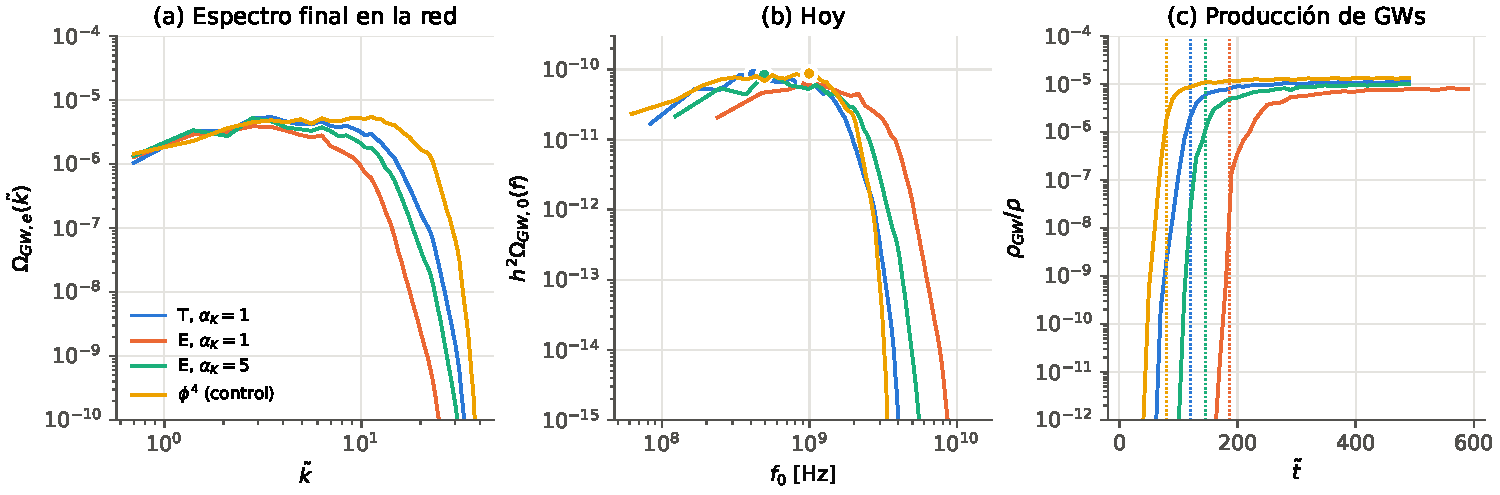
\includegraphics[width=\textwidth]{figuras/corridas_N64.pdf}
                \caption{Los cuatro casos cuárticos con $N = 64$. (a) Espectro de GWs al final de la simulación, en unidades de programa. (b) El mismo espectro llevado a hoy (Sec.~\ref{sec:reescaleo}); el punto marca el máximo. (c) Fracción de la energía en GWs; la línea punteada marca el máximo de rms$(\tilde\chi)$, es decir, cuándo la resonancia satura.}
                \label{fig:corridas-N64}
            \end{figure}

            \begin{table}[H]
                \centering
                \small
                \begin{tabular}{lcccccccc}
                    \toprule
                    caso & $f_{\text{pico}}$ [Hz] & $\tilde k_{\text{pico}}$ & $h^2\Omega_{GW,0}^{\text{pico}}$ & $\tilde k$ con $> \frac12$ pico & Hz por $\tilde k$ & $\rho_{GW}/\rho$ & $\tilde t_\chi$ & $\tilde t_{90}$ \\
                    \midrule
                    T, $\alpha_K = 1$ & $4.1 \times 10^8$ & 3.5 & $8.7 \times 10^{-11}$ & 1.4--11 & $1.19 \times 10^8$ & $1.12 \times 10^{-5}$ & 121 & 270 \\
                    E, $\alpha_K = 1$ & $9.5 \times 10^8$ & 2.8 & $6.3 \times 10^{-11}$ & 1.4--6.3 & $3.40 \times 10^8$ & $0.79 \times 10^{-5}$ & 186 & 380 \\
                    E, $\alpha_K = 5$ & $4.9 \times 10^8$ & 2.8 & $8.4 \times 10^{-11}$ & 1.4--8.4 & $1.76 \times 10^8$ & $0.99 \times 10^{-5}$ & 146 & 340 \\
                    $\phi^4$ (control) & $9.9 \times 10^8$ & 11.2 & $8.8 \times 10^{-11}$ & 2.1--17 & $0.89 \times 10^8$ & $1.36 \times 10^{-5}$ & 80 & 230 \\
                    \bottomrule
                \end{tabular}
                \caption{Resultados con $N = 64$. $\tilde t_\chi$: máximo de rms$(\tilde\chi)$; $\tilde t_{90}$: cuándo $\rho_{GW}/\rho$ llega al $90\%$ de su valor final. La columna «Hz por $\tilde k$» es el factor que lleva $\tilde k$ a $f_0$ (Sec.~\ref{sec:reescaleo}).}
                \label{tab:resultados-N64}
            \end{table}

            \paragraph{Las corridas son confiables.} En las cuatro, $\langle w\rangle$ queda a menos de $0.5\%$ de $1/3$ y el error de Friedmann es $\le 2.4 \times 10^{-3}$ (el mayor es el del monomial, que es el que más se expande). Todos los modos de GWs terminan dentro del horizonte ($k_{\text{IR}}/(aH) \ge 343$), y la integral del espectro de GWs reproduce el $\rho_{GW}/\rho$ de \CosmoLattice a $10^{-14}$. La producción está saturada: $\rho_{GW}/\rho$ crece menos de un $5\%$ en los últimos 100 de $\tilde t$. La corrida T es la de validación con otra semilla, y da el mismo $\rho_{GW}/\rho$ a un $0.2\%$ ($1.116 \times 10^{-5}$ contra $1.114 \times 10^{-5}$).

            \paragraph{En la red, los cuatro espectros son casi iguales en el IR y difieren en el UV.} Para $\tilde k \lesssim 3$ los cuatro espectros finales coinciden dentro de un factor $1.5$ ($\Omega_{GW,e} \simeq 1$--$5 \times 10^{-6}$; Fig.~\ref{fig:corridas-N64}a). Esto es lo esperable, porque en variables de programa los cuatro casos tienen el mismo potencial cerca del mínimo ($\tilde\phi^4/4$) y el mismo $q = 120$. La diferencia está en el UV: el espectro se extiende más cuanto antes satura la resonancia. El orden es el mismo en $\tilde t_\chi$ y en el corte UV: monomial ($\tilde t_\chi = 80$, el espectro supera la mitad del pico hasta $\tilde k \simeq 17$), T (121; 11), E con $\alpha_K = 5$ (146; 8.4) y E con $\alpha_K = 1$ (186; 6.3). Una explicación posible es que, al saturar antes, la cascada no lineal tiene más tiempo para llevar energía al UV; con estas cuatro corridas no lo podemos separar de otros efectos. Que la resonancia llegue antes o después tiene que ver con cuánto se aparta el arranque del régimen cuártico, pero no sólo a través de $\phi_0/M$: el E-model con $\alpha_K = 1$ ($\phi_0/M = 1.2$) es el más tardío, pero el E-model con $\alpha_K = 5$ ($\phi_0/M = 0.71$) resuena después que el T-model ($\phi_0/M = 0.79$), así que también importa la forma del potencial.

            \paragraph{Hoy, las amplitudes son parecidas y las frecuencias se separan.} Como $\epsilon = 1$ (Sec.~\ref{sec:reescaleo}), la amplitud de hoy es el $\Omega_{GW,e}$ de la red por la misma constante en los cuatro casos. Por eso los máximos quedan todos entre $6$ y $9 \times 10^{-11}$. La frecuencia, en cambio, se reescala con un factor distinto en cada caso, $\propto (\omega_*/f_*)^{1/2}/(a_e\tilde\rho_e^{1/4})$, que va de $0.89 \times 10^8$\,Hz (monomial) a $3.4 \times 10^8$\,Hz (E, $\alpha_K = 1$) por unidad de $\tilde k$. Ese factor es lo que separa las curvas de la Fig.~\ref{fig:corridas-N64}b. El T-model y el monomial tienen el mismo $\omega_*/f_*$, pero el monomial arranca con más energía en unidades de programa y se expande más antes de llegar a $w = 1/3$: su $a\tilde\rho^{1/4}$ es $1.20$ veces el del T-model al principio y $1.34$ veces al final (en radiación, $a\tilde\rho^{1/4}$ es constante). Por eso sus frecuencias quedan $1.34$ veces más bajas.

            \paragraph{La frecuencia del pico no es robusta.} Los cuatro espectros son anchos: el de hoy supera la mitad del máximo en una década de $\tilde k$ (en el monomial, de $\tilde k = 2.1$ a 17). Además, con $\tilde k_{\text{IR}} = 0.7$ los bins tienen un ancho de $20$--$25\%$ en el pico. Por eso el máximo puede caer en bins muy distintos. Por ejemplo, el monomial y el E-model con $\alpha_K = 1$ tienen el pico casi en la misma frecuencia ($\simeq 10^9$\,Hz) por razones opuestas: el monomial tiene un factor de reescaleo chico y el pico en $\tilde k = 11.2$, porque su espectro sigue plano hasta ahí, y el E-model un factor grande y el pico en $\tilde k = 2.8$. Para comparar modelos conviene usar la banda en la que el espectro supera la mitad del máximo, no la frecuencia del pico. Las corridas con $N = 128$ y $\tilde k_{\text{IR}} = 0.35$ (Sec.~\ref{sec:recomendacion}) van a resolver mejor esa zona.

    \section{Corridas cuadráticas: resultados con $N = 64$}
        \label{sec:resultados-cuadraticos}

            Corrimos los cuatro casos de la Tabla~\ref{tab:parametros-cuadraticos} con \texttt{code/correr\_cuadraticos.sh 64}. Para que sean comparables entre sí, los cuatro usan la misma grilla ($N = 64$, $\tilde k_{\text{IR}} = 3$, $\tilde k_{\max} = 166$), el mismo paso ($\delta\tilde t = 0.003$), el mismo $\tilde t_{\max} = 400$, el mismo $q = 4 \times 10^4$ y la misma semilla (\texttt{baseSeed = 20261005}). Así las fluctuaciones iniciales son la misma realización y las diferencias vienen sólo del potencial. Cada corrida tardó entre 51 y 70\,min. Los casos cuárticos de la Sec.~\ref{sec:resultados-N64} tenían semillas aleatorias distintas.

            \begin{figure}[H]
                \centering
                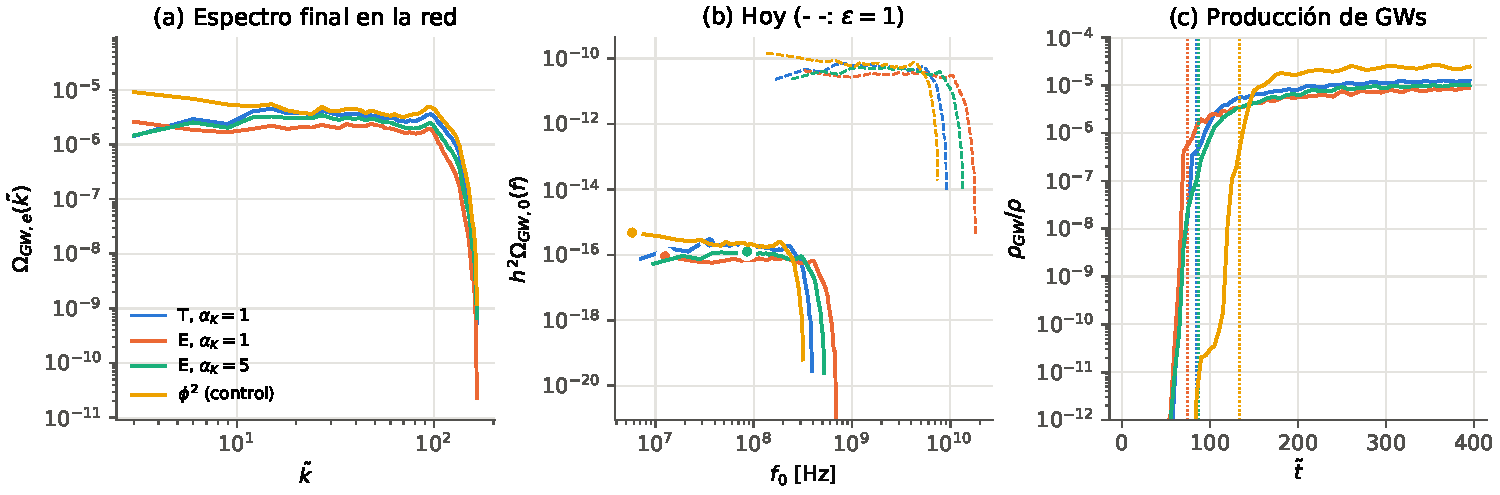
\includegraphics[width=\textwidth]{figuras/corridas_N64_cuadraticos.pdf}
                \caption{Los cuatro casos cuadráticos con $N = 64$ y la misma semilla. (a) Espectro de GWs al final de la simulación. (b) Llevado a hoy con $T_{\text{RH}} = 10^{10}$\,GeV y $w = 0$ hasta el reheating (línea llena; el punto marca el máximo), y con $\epsilon = 1$, radiación desde el final de la simulación (línea cortada). (c) Fracción de la energía en GWs; la línea punteada marca cuándo rms$(\tilde\chi)$ llega a la mitad de su máximo.}
                \label{fig:corridas-cuadraticos}
            \end{figure}

            \begin{table}[H]
                \centering
                \footnotesize
                \setlength{\tabcolsep}{3pt}
                \begin{tabular}{lccccccc}
                    \toprule
                    caso & $\rho_{GW}/\rho$ & crece & $\langle w\rangle_e$ & $h^2\Omega^{\max}_{GW,0}$ ($w{=}0$) & banda ($w{=}0$) [Hz] & $h^2\Omega^{\max}_{GW,0}$ ($\epsilon{=}1$) & $\epsilon$ \\
                    \midrule
                    T, $\alpha_K = 1$ & $1.23 \times 10^{-5}$ & $10\%$ & $0.27$ & $2.4 \times 10^{-16}$ & $1.4 \times 10^7$--$2.6 \times 10^8$ & $7.3 \times 10^{-11}$ & $3.3 \times 10^{-6}$ \\
                    E, $\alpha_K = 1$ & $0.89 \times 10^{-5}$ & $26\%$ & $0.29$ & $0.9 \times 10^{-16}$ & $1.3 \times 10^7$--$4.3 \times 10^8$ & $4.2 \times 10^{-11}$ & $2.1 \times 10^{-6}$ \\
                    E, $\alpha_K = 5$ & $1.02 \times 10^{-5}$ & $16\%$ & $0.26$ & $1.3 \times 10^{-16}$ & $1.9 \times 10^7$--$3.2 \times 10^8$ & $5.5 \times 10^{-11}$ & $2.3 \times 10^{-6}$ \\
                    $\phi^2$ (control) & $2.46 \times 10^{-5}$ & $4\%$ & $0.25$ & $4.8 \times 10^{-16}$ & $5.8 \times 10^6$--$1.9 \times 10^8$ & $1.5 \times 10^{-10}$ & $3.3 \times 10^{-6}$ \\
                    \bottomrule
                \end{tabular}
                \caption{Resultados cuadráticos con $N = 64$. «Crece»: aumento de $\rho_{GW}/\rho$ en los últimos 100 de $\tilde t$. $\langle w\rangle_e$: promedio en los dos últimos períodos. La banda es donde el espectro de hoy supera la mitad de su máximo. $\epsilon = a_e/a_{RD}$ para $T_{\text{RH}} = 10^{10}$\,GeV y $w = 0$.}
                \label{tab:resultados-cuadraticos}
            \end{table}

            \paragraph{Las corridas son numéricamente buenas.} El error de Friedmann es $\le 9 \times 10^{-5}$ en las cuatro, la integral del espectro de GWs reproduce $\rho_{GW}/\rho$ a $10^{-14}$ y todos los modos terminan dentro del horizonte ($k_{\text{IR}}/(aH) \ge 39$).

            \paragraph{El condensado se fragmenta casi por completo.} En los cuatro casos, $\langle\tilde\phi\rangle a^{3/2}$ (que sin resonancia oscilaría con amplitud constante) cae a la mitad entre $\tilde t \simeq 108$ y $140$. Al final queda entre el $0.2\%$ y el $3\%$ de su amplitud inicial.

            \paragraph{Por qué $\langle w\rangle$ no es 0.} Para un potencial cuadrático, $w = 0$ vale para el condensado homogéneo oscilando: por el teorema del virial, la presión promediada en una oscilación se anula. En las corridas eso se cumple antes de la resonancia, pero deja de valer cuando el condensado se fragmenta:
            \begin{table}[H]
                \centering
                \small
                \begin{tabular}{lccccc}
                    \toprule
                    caso & $\tilde t = 20$--$50$ & $100$--$150$ & $200$--$250$ & $350$--$400$ & gradientes / total (final) \\
                    \midrule
                    T, $\alpha_K = 1$ & $0.028$ & $0.149$ & $0.239$ & $0.265$ & $37\%$ \\
                    E, $\alpha_K = 1$ & $0.016$ & $0.130$ & $0.219$ & $0.280$ & $38\%$ \\
                    E, $\alpha_K = 5$ & $0.026$ & $0.125$ & $0.225$ & $0.268$ & $36\%$ \\
                    $\phi^2$ (control) & $0.029$ & $0.043$ & $0.238$ & $0.250$ & $33\%$ \\
                    \bottomrule
                \end{tabular}
                \caption{$\langle w\rangle$ promediado en ventanas de $\tilde t$, y fracción de la energía total que está en gradientes al final de cada corrida cuadrática.}
                \label{tab:w-cuadraticos}
            \end{table}
            Antes de la resonancia $\langle w\rangle \simeq 0.02$--$0.03$. Lo esperable es 0; la diferencia probablemente viene de que la ventana no abarca un número entero de oscilaciones y de que al principio la expansión no es despreciable frente a la frecuencia de oscilación. Después, $w$ sube hasta $0.25$--$0.29$, en el monomial más tarde porque resuena más tarde. El mecanismo es el siguiente:
            \begin{itemize}
                \item \textbf{La energía pasa a modos con momento alto.} La resonancia y la cascada no lineal que la sigue pasan la energía del condensado ($k = 0$) a fluctuaciones de $\chi$ y de $\phi$ con momentos comparables o mayores que la masa. Al final, la mitad de la energía de gradiente de cada campo está en $\tilde k \gtrsim 60$--$100$, es decir, con momento físico $p/m = \tilde k/a \simeq 1.5$--$2.5$ (con la masa desnuda $m = \omega_*$). Esas partículas son semirrelativistas y su presión se acerca a la de la radiación.
                \item \textbf{No llega a $1/3$} porque parte de la energía sigue en modos no relativistas (restos del condensado y partículas con $p \lesssim m$) y porque las masas efectivas inducidas por la interacción ($g^2\langle\chi^2\rangle$ para $\phi$, $g^2\langle\phi^2\rangle$ para $\chi$) son apreciables.
            \end{itemize}
            Es lo mismo que encontraron Podolsky, Felder, Kofman \& Peloso para $m^2\phi^2/2 + g^2\phi^2\chi^2/2$ en simulaciones en la red (Phys.\ Rev.\ D \textbf{73}, 023501 (2006), arXiv:hep-ph/0507096, Sec.~III.B y Fig.~1): $w$ pasa bruscamente de $0$ a $\sim 0.2$--$0.3$ al final del preheating, en $t \sim 100$--$150/m$, y no llega enseguida a $1/3$. Según los autores, esto se debe en parte a que justo después del preheating el campo liviano todavía tiene una masa efectiva inducida importante, y en parte a la contribución residual del inflatón homogéneo. Dufaux \emph{et al.}\ (arXiv:0707.0875, Sec.~III.D) toman ese mismo resultado como punto de partida del reescaleo a hoy.

            \paragraph{Qué pasa después de la simulación.} El valor $w \simeq 0.25$ no debería mantenerse. El momento físico de cada partícula cae como $1/a$, así que, si el inflatón no decae antes, sus partículas se vuelven no relativistas cuando el universo se expande otro factor $\sim 2$--$3$ (con las estimaciones de arriba) y $w$ vuelve a bajar hacia 0. Podolsky \emph{et al.}\ (Sec.~III.B, punto iii) lo argumentan así para un inflatón masivo: aun en minoría al final del preheating, sus partículas terminan dominando y el universo vuelve a estar dominado por materia. Lozanov \& Amin (Phys.\ Rev.\ Lett.\ \textbf{119}, 061301 (2017), arXiv:1608.01213) encuentran lo mismo en simulaciones de la fragmentación del inflatón sin campo hijo: para $V \propto |\phi|^{2n}$ cerca del mínimo, a tiempos largos $w \to 0$ si $n = 1$ y $w \to 1/3$ para $n$ mayores (modelos de un solo campo, con simulaciones en la red). Para el caso cuártico ($n = 2$ en su notación) esto es consistente con $w = 1/3$ y con que $\epsilon = 1$ (Sec.~\ref{sec:reescaleo}). La evolución completa de $w$ requiere simular más tiempo o seguir fuera de la red la energía de cada modo, $\sqrt{p^2 + m^2}$ con $p \propto 1/a$. Hasta tener eso, el resultado de hoy queda acotado entre $w = 0$ desde $a_e$ y $w \simeq 0.25$ constante.

            \paragraph{El orden es el inverso del caso cuártico.} Las GWs empiezan a crecer ($\rho_{GW}/\rho = 10^{-8}$) en $\tilde t \simeq 70$ (E, $\alpha_K = 1$), $75$ (T y E con $\alpha_K = 5$) y $120$ (monomial). En el caso cuártico el monomial era el primero en resonar (Sec.~\ref{sec:resultados-N64}). Aun así, el monomial termina con más GWs: $\rho_{GW}/\rho = 2.5 \times 10^{-5}$, el doble que el T-model, con más potencia en el IR ($\Omega_{GW,e} \simeq 0.9 \times 10^{-5}$ en $\tilde k = 3$, contra $1.4$--$2.6 \times 10^{-6}$). Con una sola semilla por caso no podemos decir si esa diferencia es mayor que la variación entre realizaciones.

            \paragraph{En la red, la producción es como la del caso cuártico.} $\rho_{GW}/\rho \simeq 1$--$2.5 \times 10^{-5}$, y el espectro final es plano ($\Omega_{GW,e} \simeq 1$--$5 \times 10^{-6}$) desde $\tilde k \simeq 3$ hasta $\tilde k \simeq 100$ (Fig.~\ref{fig:corridas-cuadraticos}a). Hay dos limitaciones:
            \begin{itemize}
                \item \textbf{El UV no está resuelto.} El espectro sigue plano hasta muy cerca de $\tilde k_{\max} = 166$, y la cola de GWs en $\tilde k_{\max}$ es $\sim 10^{-4}$ del máximo. Con $N = 32$ ($\tilde k_{\max} = 83$) el T-model daba un máximo en $\tilde k \simeq 50$, cerca de su propio corte, y $\rho_{GW}/\rho = 1.7 \times 10^{-5}$ ($28\%$ más). La forma del espectro por encima de $\tilde k \sim 50$ depende entonces de la resolución, y el máximo no tiene sentido: cae en el primer bin o en cualquier punto de la meseta. Para resolver el UV hace falta $N = 128$ con el mismo $\tilde k_{\text{IR}}$, unas 9\,h por corrida.
                \item \textbf{La producción no terminó del todo.} $\rho_{GW}/\rho$ crece entre un $4\%$ y un $26\%$ en los últimos 100 de $\tilde t$. Con $w \simeq 0.25$, sin fuente ese cociente bajaría como $a^{-0.25}$, así que todavía se producen GWs. Los valores finales son entonces cotas inferiores, con un margen de $\sim 10$--$30\%$.
            \end{itemize}

            \paragraph{Hoy, lo que manda es la historia después de la simulación.} Con $T_{\text{RH}} = 10^{10}$\,GeV y $w = 0$ hasta el reheating, $\epsilon = 2$--$3 \times 10^{-6}$. La meseta queda en $h^2\Omega_{GW,0} \sim 10^{-16}$ (máximos de $0.9$ a $4.8 \times 10^{-16}$), entre $6 \times 10^6$ y $4 \times 10^8$\,Hz. Con $\epsilon = 1$ los mismos espectros dan $4 \times 10^{-11}$--$1.5 \times 10^{-10}$ entre $10^8$ y $2 \times 10^{9}$\,Hz, del mismo orden que el caso cuártico. Si $w$ se quedara en el valor medido al final ($\simeq 0.25$) hasta el reheating, $\epsilon \simeq 0.07$--$0.08$ y los máximos serían $3$--$12 \times 10^{-12}$ (\texttt{--w\_post 0.25}). Ninguno de los extremos es realista:
            \begin{itemize}
                \item $w = 0$ desde $a_e$ ignora que el inflatón ya está fragmentado;
                \item $w \simeq 0.25$ constante ignora que las partículas de $\phi$ y $\chi$, que tienen masa, se vuelven no relativistas a medida que el universo se expande, y entonces $w$ vuelve a bajar.
            \end{itemize}
            El valor real está entre los dos y requiere seguir la evolución de $w$ más allá de la simulación. Lo robusto es la comparación con el caso cuártico: la producción en la red es parecida, y lo que separa a los modelos cuadráticos (hasta cinco órdenes de magnitud abajo) es la expansión tipo materia hasta el reheating, que no existe para $n = 4$.

    \section{Guía de uso: los cuatro casos, sus parámetros y cómo correrlos}
        \label{sec:guia}

        \subsection{Los cuatro casos}

            \begin{table}[H]
                \centering
                \footnotesize
                \setlength{\tabcolsep}{3pt}
                \begin{tabular}{lcccc}
                    \toprule
                    & T, $\alpha_K = 1$ & E, $\alpha_K = 5$ & E, $\alpha_K = 1$ & monomial (control) \\
                    \midrule
                    archivo \texttt{.in} & \texttt{gentmodel\_cuartico} & \texttt{genemodel\_cuartico\_aK5} & \texttt{genemodel\_cuartico} & \texttt{genmonomial\_cuartico} \\
                    ejecutable & \texttt{gentmodel} & \texttt{genemodel} & \texttt{genemodel} & \texttt{genmonomial} \\
                    $V(\phi)$ & $A\tanh^4(\phi/M)$ & $A(1-e^{-\phi/M})^4$ & $A(1-e^{-\phi/M})^4$ & $A\phi^4$ \\
                    \texttt{M} [GeV] & $5.96451 \times 10^{18}$ & $6.66852 \times 10^{18}$ & $2.98225 \times 10^{18}$ & -- \\
                    \texttt{A} [GeV$^4$ o adim.] & $4.21854 \times 10^{63}$ & $1.87750 \times 10^{64}$ & $4.02858 \times 10^{63}$ & $3.33322 \times 10^{-12}$ \\
                    $\phi_0 = f_*$ [GeV] & $4.69413 \times 10^{18}$ & $4.73073 \times 10^{18}$ & $3.56906 \times 10^{18}$ & $6.88722 \times 10^{18}$ \\
                    $\dot\phi_0$ [GeV$^2$] & $-2.0345 \times 10^{31}$ & $-2.5689 \times 10^{31}$ & $-2.2449 \times 10^{31}$ & $-6.2899 \times 10^{31}$ \\
                    $\omega_*$ [GeV] & $1.714 \times 10^{13}$ & $2.915 \times 10^{13}$ & $5.094 \times 10^{13}$ & $2.515 \times 10^{13}$ \\
                    $\omega_*/f_* = \sqrt{\lambda_{\text{eff}}}$ & $3.651 \times 10^{-6}$ & $6.163 \times 10^{-6}$ & $1.427 \times 10^{-5}$ & $3.651 \times 10^{-6}$ \\
                    $q$ & 120 & 120 & 120 & 120 \\
                    \texttt{tMax} & 500 & 500 & 600 & 500 \\
                    $n_s$, $r$ & 0.964, 0.004 & 0.965, 0.015 & 0.965, 0.004 & 0.946, 0.29 (excluido) \\
                    \bottomrule
                \end{tabular}
                \caption{Los cuatro casos cuárticos ($n = 4$, por lo tanto $\alpha = 1$ en \CosmoLattice). En los tres primeros, \texttt{A} está en GeV$^4$ porque multiplica una función adimensional; en el monomial es adimensional ($V = A\phi^4$). Todos los valores los recalcula \texttt{code/parametros\_cuarticos.py}, que además comprueba que coinciden con los \texttt{.in}.}
                \label{tab:casos}
            \end{table}

        \subsection{Cada parámetro de los \texttt{.in}}

            Todos los \texttt{.in} cuárticos tienen las mismas claves. Las que no aparecen toman el valor por defecto de \CosmoLattice (\texttt{include/CosmoInterface/runparameters.h}). Cualquiera se puede cambiar desde la terminal sin editar el archivo, agregando \texttt{clave=valor} al comando (ver la Sec.~\ref{sec:terminal}).

            \paragraph{Salida.}
            \begin{description}
                \item[\texttt{outputfile = ./}] Directorio donde se escriben los archivos de salida, relativo al directorio desde el que se lanza el ejecutable.
                \item[\texttt{print\_headers = true}] Escribe una línea de encabezado con el nombre de cada columna. El analizador la usa para identificar las columnas.
                \item[\texttt{overwriteFiles = false}] Si en el directorio ya hay una salida, \CosmoLattice se niega a pisarla. Para repetir una corrida, pasar \texttt{overwriteFiles=true} (el script lo hace solo).
            \end{description}

            \paragraph{Evolución.}
            \begin{description}
                \item[\texttt{expansion = true}] Expansión autoconsistente: $a(\tilde t)$ se evoluciona con las ecuaciones de Friedmann, usando la energía de los campos.
                \item[\texttt{evolver = VV2}] Velocity-Verlet de segundo orden para los escalares. Las GWs se evolucionan con leapfrog (\texttt{doLFforGWs = true} por defecto). Error de Friedmann $\propto \delta\tilde t^{\,2}$ (Sec.~\ref{sec:dt}).
            \end{description}

            \paragraph{Grilla.}
            \begin{description}
                \item[\texttt{N = 64}] Puntos por lado; hay $N^3$ sitios. Fija la memoria ($\simeq 10\,\text{MB} + 148\,\text{B} \times N^3$) y el tiempo ($\propto N^3$). Ver la Tabla~\ref{tab:recursos}.
                \item[\texttt{dt = 0.01}] Paso temporal en tiempo de programa $\tilde t$. Es estable y está convergido hasta $N = 192$ (Sec.~\ref{sec:dt}).
                \item[\texttt{kIR = 0.7}] Momento más chico de la caja, en unidades de $\omega_*$. El lado de la caja es $\tilde L = 2\pi/\tilde k_{\text{IR}} \simeq 9$, el momento máximo es $\tilde k_{\max} = \sqrt 3 N \tilde k_{\text{IR}}/2$ (39 para $N = 64$) y el ancho de los bins de los espectros es $\tilde k_{\text{IR}}$. Al subir $N$, conviene bajarlo como $0.7 \times 64/N$.
            \end{description}

            \paragraph{Tiempos de salida} (en $\tilde t$).
            \begin{description}
                \item[\texttt{tOutputFreq = 0.2}] Cada cuánto se escriben los promedios (\texttt{average\_*.txt}: fondo, campos, energías, Friedmann). Tiene que resolver la oscilación del inflatón (período $\tilde T \simeq 6$--$10$), porque el analizador promedia $w$ por períodos y deriva con splines.
                \item[\texttt{tOutputInfreq = 10}] Cada cuánto se escriben los espectros de los campos y de GWs (\texttt{spectra\_*.txt}). Cada uno cuesta $\sim 3$ pasos, así que bajarlo a 5 es barato si se quieren más curvas.
                \item[\texttt{tOutputRareFreq = 50}] Cada cuánto se toman instantáneas 3D de la energía. Sólo actúa si se piden instantáneas (claves \texttt{snapshots}, que no usamos).
                \item[\texttt{tMax}] Tiempo final. Es 500 o 600 (Tabla~\ref{tab:casos}), elegido para que $\rho_{GW}/\rho$ haya saturado (Sec.~\ref{sec:in}).
            \end{description}

            \paragraph{Espectros.}
            \begin{description}
                \item[\texttt{PS\_type = 1}] Espectro de tipo~I: suma sobre los modos de cada bin con su multiplicidad exacta. Captura mejor la cola UV que el tipo~II (nota técnica~II de \CosmoLattice, Sec.~4.1).
                \item[\texttt{PS\_version = 1}] Reescalea cada bin por su valor central.
            \end{description}

            \paragraph{Condiciones iniciales.}
            \begin{description}
                \item[\texttt{kCutOff = 18}] Las fluctuaciones cuánticas iniciales se siembran sólo en $\tilde k < 18$. Así se evita que el ruido de vacío de los modos UV, que no tiene significado físico en la grilla, genere GWs espurias. La resonancia está en $\tilde k \sim 1$--$10$.
                \item[\texttt{initial\_amplitudes = $\phi_0$ 0}] Valor homogéneo inicial de $\phi$ y de $\chi$ en GeV. El primero fija $f_* = \phi_0$. Viene de $\epsilon_V = 1$ (Sec.~\ref{sec:ci}).
                \item[\texttt{initial\_momenta = $\dot\phi_0$ 0}] Velocidades homogéneas iniciales en GeV$^2$: slow-roll con $H$ autoconsistente (Sec.~\ref{sec:momento-inicial}).
                \item[\texttt{baseSeed}] (no está en los \texttt{.in}) Semilla de las fluctuaciones iniciales. Si no se da, es aleatoria y cada corrida es una realización distinta: de ahí la dispersión de $\pm 10\%$ en $\rho_{GW}/\rho$ de la Sec.~6.4. Para comparar corridas que difieren en un solo parámetro conviene fijarla (\texttt{baseSeed=1234}).
            \end{description}

            \paragraph{Modelo.}
            \begin{description}
                \item[\texttt{n = 4}] Potencia del potencial. Fija $\alpha = 3(n-2)/(n+2) = 1$ y la ecuación de estado $w = 1/3$.
                \item[\texttt{M}] Escala del T/E-model en GeV: $\sqrt{6\alpha_K}\,m_p$ (T) o $\sqrt{3\alpha_K/2}\,m_p$ (E). No aparece en el monomial.
                \item[\texttt{A}] Altura del potencial, $A = \tfrac34 \lambda m_p^4$ con $\lambda$ normalizado al CMB (Sec.~\ref{sec:parametros-cuarticos}). En el monomial, $A = \lambda_{\text{eff}}/4$.
                \item[\texttt{q = 120}] Parámetro de resonancia $q = g^2\phi_0^2/\omega_*^2 = g^2/\lambda_{\text{eff}}$ para el acople $\tfrac12 g^2\phi^2\chi^2$. El paper no lo fija: 120 es el valor de Dufaux \emph{et al.}
            \end{description}

            \paragraph{GWs.}
            \begin{description}
                \item[\texttt{withGWs = true}] Evoluciona las perturbaciones tensoriales $h_{ij}$, que duplica la memoria y suma $\sim 70\%$ al tiempo por paso, y escribe \texttt{spectra\_energy\_gws.txt} y \texttt{average\_energies\_gws.txt}.
                \item[\texttt{GWprojectorType = 1}] Proyector transverso-sin-traza construido con el momento de red $k_L = k_L^0$ (derivada centrada). Las tres opciones dan espectros casi idénticos salvo en la cola UV (nota técnica~II, Sec.~4.1).
            \end{description}

        \subsection{Cómo correrlo desde la terminal}
            \label{sec:terminal}

            Todos los comandos se escriben desde la raíz del repositorio (\texttt{CL\_GWs/}).

            \paragraph{1. Estimar memoria y tiempo antes de lanzar.}
            {\footnotesize\begin{verbatim}
python3 code/recursos_cosmolattice.py --kmax-fijo --N 64 128 192 --tMax 500
            \end{verbatim}}
            Imprime $\delta\tilde t$, memoria, segundos por paso y horas totales, y avisa si no entra en la memoria libre.

            \paragraph{2a. Correr los casos con el script (recomendado).}
            {\footnotesize\begin{verbatim}
code/correr_cuarticos.sh                 # los 3 del paper, N = 64 (~1.5 h)
code/correr_cuarticos.sh 128             # N = 128, kIR = 0.35 (~13 h)
CONTROL=1 code/correr_cuarticos.sh 64    # los 3 + el monomial de control (~2 h)
MODELOS="genmonomial_cuartico" code/correr_cuarticos.sh 64   # sólo el control
nohup code/correr_cuarticos.sh 128 > corridas_N128.log 2>&1 &  # sigue al cerrar la terminal
            \end{verbatim}}
            El script compila los ejecutables que falten y verifica la memoria antes de empezar. Después corre los casos uno por uno: cada uno usa los 8 hilos, así que correrlos a la vez no ahorra tiempo. Saltea los que ya terminaron (\texttt{FORZAR=1} para repetirlos) y analiza cada uno al terminar. Otras opciones: un segundo argumento para \texttt{kIR}, \texttt{DT=0.007}, \texttt{NTHREADS=4} y \texttt{EXTRA\_ARGS="baseSeed=1234 tMax=300"}. Las salidas quedan en \texttt{build\_corridas/<caso>\_N<N>\_kIR<kIR>/}, y los tiempos reales en \texttt{build\_corridas/tiempos.txt}.

            \paragraph{2b. Correr un caso a mano.}
            {\footnotesize\begin{verbatim}
# compilar (una vez por modelo)
mkdir -p build_genmonomial && cd build_genmonomial
cmake .. -DMODEL=genmonomial -DCMAKE_BUILD_TYPE=Release && make -j4
# correr (desde un directorio propio, porque escribe la salida en ./)
mkdir -p corrida_N64 && cd corrida_N64
OMP_NUM_THREADS=8 ../genmonomial input=../../models/parameter-files/genmonomial_cuartico.in
# cualquier parámetro del .in se puede pisar en la línea de comandos:
OMP_NUM_THREADS=8 ../genmonomial input=../../models/parameter-files/genmonomial_cuartico.in \
    N=128 kIR=0.35 baseSeed=1234 overwriteFiles=true
            \end{verbatim}}

            \paragraph{3. Seguir una corrida en curso.}
            {\footnotesize\begin{verbatim}
tail -f build_corridas/gentmodel_cuartico_N64_kIR0.7/salida.log   # "Step ... Current time: t~"
tail -f corridas_N128.log                                         # progreso del script
free -h                                                           # memoria libre
            \end{verbatim}}

            \paragraph{4. Analizar.}
            {\footnotesize\begin{verbatim}
python3 code/analisis_cosmolattice.py build_corridas/gentmodel_cuartico_N64_kIR0.7
            \end{verbatim}}
            Los gráficos y el \texttt{resumen.txt} quedan en \texttt{analisis/} dentro de cada corrida (Sec.~\ref{sec:analisis}). Para comparar el control con el T-model, hay que mirar los \texttt{05\_gws.png} y \texttt{06\_energias.png} de las dos corridas con la misma $N$ y \texttt{kIR}, idealmente con la misma \texttt{baseSeed}.

    % Secciones de cada modelo: sólo existen en su rama (monomial, t-model, e-model).
    \IfFileExists{modelos/monomial.tex}{    \section{Modelo monomial: $V = A|\phi|^n$}
        \label{sec:monomial}

        Implementado en \texttt{models/genmonomial.h}; los \texttt{.in} son \texttt{genmonomial.in} ($n = 6$, exploratorio) y \texttt{genmonomial\_cuartico.in} (el control cuártico de la Sec.~\ref{sec:control}). Para este potencial $A_{\text{eff}} = A$ en el marco común (Sec.~\ref{sec:marco}).

        \subsection{Derivadas}

        \subsection{Derivadas}

            Consideremos que los potenciales monomiales generales para el potencial son de la forma
            \begin{equation}
                V(\phi) = A \left| \phi \right|^n
            \end{equation}
            El valor absoluto es necesario para que $V$ esté bien definido en $\phi < 0$ cuando $n$ no es un entero par.

            Para la implementación de estos modelos en \CosmoLattice debemos calcular sus derivadas primera y segunda:
            \begin{equation}
                V^\prime (\phi) = A n \operatorname{sgn}(\phi) \left| \phi \right|^{n - 1} = A n \, \phi \left| \phi \right|^{n - 2}
            \end{equation}
            \begin{equation}
                V^{\prime \prime} (\phi) = A n (n - 1) \left| \phi \right|^{n - 2}
            \end{equation}
            (para $n < 2$ ambas divergen en $\phi = 0$, y la expresión $\phi |\phi|^{n-2}$ del código da $0 \cdot \infty$ en ese punto).

        \subsection{Variables de programa}

            Con $A_{\text{eff}} = A$ (Sec.~\ref{sec:variables}): $\omega_* = \sqrt{nA}\,\phi_0^{n/2-1}$, $q = g^2\phi_0^{4-n}/(nA)$ y $\tilde V = |\tilde\phi|^n/n + \tfrac12 q\tilde\phi^2\tilde\chi^2$ exactamente (no sólo cerca del mínimo). Con $n = 4$ y $A = \lambda/4$ es \texttt{lphi4}.

        \subsection{Condiciones iniciales y momento inicial}

            Planteemos la condición inicial del campo como aquella tal que $\epsilon = 1$.
            \begin{equation*}
                \begin{split}
                    \epsilon &= \frac{m_p^2}{2} \left[ \frac{V^\prime (\phi)}{V(\phi)} \right]^2\\
                    1 &= \frac{m_p^2}{2} \left[ \frac{V^\prime (\phi_0)}{V(\phi_0)} \right]^2\\
                    \frac{2}{m_p^2} &= \left[ \frac{A n \phi^{n-1}_0}{A \phi^n_0} \right]^2\\
                    \frac{\sqrt{2}}{m_p} &= \frac{n}{\phi_0}\\
                    \phi_0 &= \frac{n}{\sqrt{2}} m_p
                \end{split}
            \end{equation*}
            \begin{equation}
                \phi_0 = \frac{\sqrt{2}}{2} n m_p
            \end{equation}
            Con la fórmula de la Sec.~\ref{sec:momento-inicial} y los parámetros de \texttt{genmonomial.in} ($n = 6$), $\dot\phi_0 = -3.063 \times 10^{31}\,\text{GeV}^2$. Integrando el fondo exacto, $\epsilon_H = 1$ se alcanza en $\phi = 9.04 \times 10^{18}\,\text{GeV}$, contra $\phi_0 = 1.033 \times 10^{19}\,\text{GeV}$.

        \subsection{Ejemplo de inestabilidad con $n = 6$}

            Con las cotas de la Sec.~\ref{sec:estabilidad}, para $n = 6$ ($\alpha = 3/2$), con $N = 64$, $\tilde k_{\text{IR}} = 3$, $\delta\tilde t = 10^{-3}$ y $q = 10^2$, las cotas dan $a_{\max}^{\text{grad}} \simeq 357$ y $a_{\max}^{\text{hijo}} \sim 1170$. En la simulación, la corrida explota en $a \simeq 290$ ($\tilde t \simeq 27$), del orden de la cota del gradiente; por eso \texttt{genmonomial.in} usa $\tilde t_{\max} = 20$ ($a \simeq 190$). Con los parámetros originales ($q = 4 \times 10^4$, $\delta\tilde t = 5 \times 10^{-3}$) la corrida explotaba ya en $\tilde t \simeq 0.5$.

        \subsection{El monomial de control}
            \label{sec:control}

            \texttt{genmonomial\_cuartico.in} \textbf{no es un modelo del paper}: $\lambda\phi^4/4$ como modelo de inflación predice $n_s = 1 - 3/(N_*+1) = 0.946$ y $r = 16/(N_*+1) = 0.29$ para $N_* = 55$ (slow-roll, con $\phi_*^2 = 8(N_*+1)\,m_p^2$), y la cota $r < 0.036$ lo excluye. Lo incluimos para separar qué parte de la señal viene del plateau de los $\alpha$-attractors:
            \begin{itemize}
                \item Usa el $\lambda_{\text{eff}} = 4A_T/M_T^4 = 1.333 \times 10^{-11}$ del T-model, con $A = \lambda_{\text{eff}}/4$. Así, cerca del mínimo tiene el mismo potencial físico que el T-model. Con el mismo $q$ tiene además el mismo acople físico, $g = \sqrt{q\lambda_{\text{eff}}}$, y el mismo $\omega_*/f_*$.
                \item La condición inicial es la de las Secs.~\ref{sec:ci}--\ref{sec:momento-inicial} ($\epsilon_V = 1$): $\phi_0 = 2\sqrt 2\, m_p$. Es mayor que la del T-model, porque sin plateau el slow-roll termina más arriba. En variables de programa los dos arrancan en $\tilde\phi = 1$, pero el monomial lo hace con más energía y más expansión inicial ($a'/a = 0.92$ contra $0.44$).
                \item Es idéntico a \texttt{lphi4} con $\lambda = \lambda_{\text{eff}}$ (Sec.~\ref{sec:variables}), así que también sirve como puente con la comparación con Dufaux \emph{et al.}\ de la Sec.~\ref{sec:literatura}.
            \end{itemize}
            Con $N = 32$ la resonancia llega antes que en el T-model: el campo hijo satura en $\tilde t \simeq 80$, contra $110$ en el T-model, y $\rho_{GW}/\rho$ alcanza el $90\%$ de su valor final en $\tilde t \simeq 230$. El valor final es $2.3 \times 10^{-5}$, contra $1.8 \times 10^{-5}$ en el T-model con la misma $N$. Hay dos cosas a tener en cuenta:
            \begin{itemize}
                \item Como $a'/a(0) = 0.92 > \tilde k_{\text{IR}} = 0.7$, los modos más IR arrancan fuera del horizonte (al final $k_{\text{IR}}/(aH) = 343$). Por lo tanto no conviene bajar $\tilde k_{\text{IR}}$ por debajo de $\sim 0.35$ en este caso.
                \item Con $N = 32$ la cola UV del inflatón es $\sim 10^{-3}$, peor que en los T/E-models, así que hay que correrlo con $N \ge 64$.
            \end{itemize}

        \subsection{Resultados con $N = 64$}
            \label{sec:monomial-N64}

            La comparación con los otros casos está en la Sec.~\ref{sec:resultados-N64}; acá van las figuras de la corrida \texttt{genmonomial\_cuartico.in}, que salen de \texttt{code/analisis\_cosmolattice.py} (las cuatro restantes, \texttt{01\_fondo}, \texttt{03\_espectros\_campos}, \texttt{04\_errores} y \texttt{06\_energias}, quedan en \texttt{build\_corridas/<caso>\_N64\_kIR0.7/analisis/}).

            \begin{figure}[H]
                \centering
                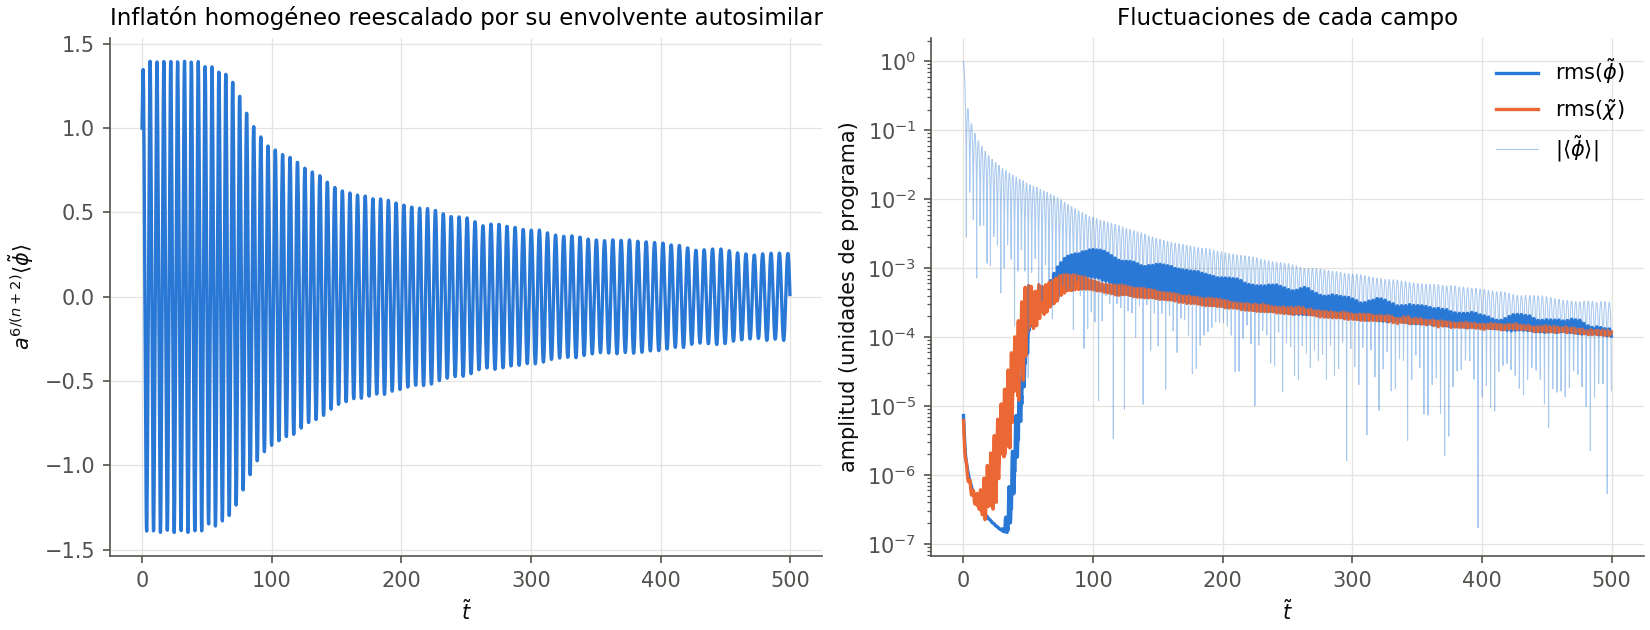
\includegraphics[width=\textwidth]{figuras/genmonomial_cuartico_N64_campos.png}
                \caption{Monomial de control ($\phi^4$), $N = 64$. Izquierda: $\langle\tilde\phi\rangle$ multiplicado por $a^{6/(n+2)} = a$, que sería una oscilación de amplitud constante sin resonancia. Derecha: rms de cada campo y $|\langle\tilde\phi\rangle|$.}
                \label{fig:genmonomial_cuartico-campos}
            \end{figure}
            \begin{figure}[H]
                \centering
                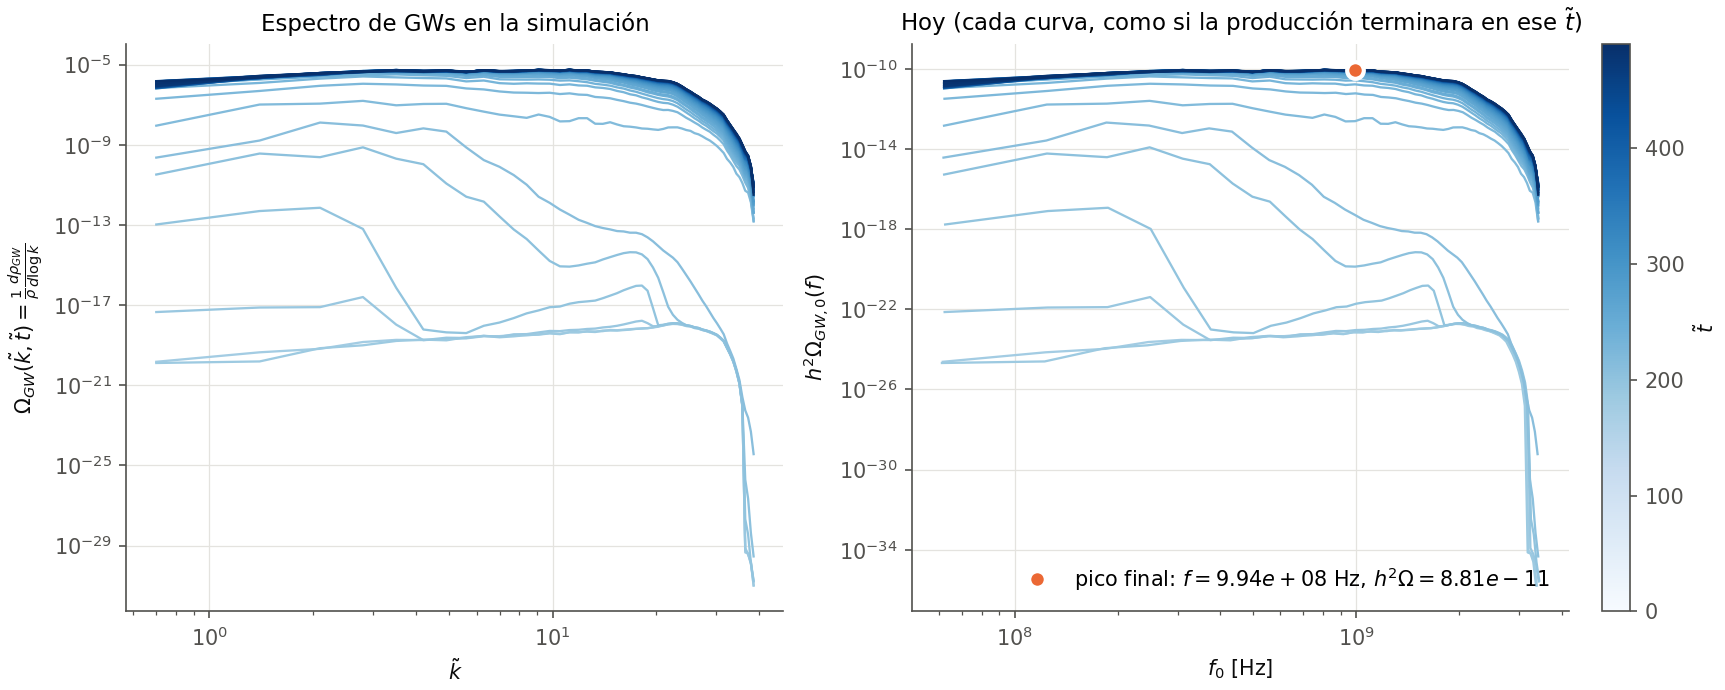
\includegraphics[width=\textwidth]{figuras/genmonomial_cuartico_N64_gws.png}
                \caption{Monomial de control ($\phi^4$), $N = 64$. Espectro de GWs en la red (izquierda) y llevado a hoy (derecha), a cada tiempo de salida (claro = temprano).}
                \label{fig:genmonomial_cuartico-gws}
            \end{figure}

            Con $N = 64$ se confirma lo que se vio con $N = 32$ (Sec.~\ref{sec:control}): sin plateau la resonancia llega antes que en cualquier $\alpha$-attractor. El rms del campo hijo es máximo en $\tilde t = 80$ (T-model: 121), y $\rho_{GW}/\rho$ llega al $90\%$ de su valor final en $\tilde t = 230$. Antes de la resonancia, $\langle\tilde\phi\rangle a$ oscila con amplitud $\simeq 1.4$ (Fig.~\ref{fig:genmonomial_cuartico-campos}), mayor que en el T-model. Es la amplitud que corresponde a arrancar con más energía cinética ($a'/a = 0.92$ contra $0.44$).

            El valor final es $\rho_{GW}/\rho = 1.36 \times 10^{-5}$, contra $2.3 \times 10^{-5}$ con $N = 32$: baja un $40\%$, igual que en el T-model. Es el caso con más potencia UV: el espectro supera la mitad del máximo de $\tilde k = 2.1$ a $17$, y por eso el máximo cae en $\tilde k = 11.2$ (Fig.~\ref{fig:genmonomial_cuartico-gws}). Como el espectro es casi plano en esa banda, la posición del máximo no es robusta (Sec.~\ref{sec:resultados-N64}). Hoy da $h^2\Omega_{GW,0} = 8.8 \times 10^{-11}$ en $9.9 \times 10^8$\,Hz, con más de la mitad del máximo entre $1.9 \times 10^8$ y $1.5 \times 10^9$\,Hz. Es la misma banda que el T-model, aunque el monomial tiene más potencia en $\tilde k$ alto, porque su factor de reescaleo es $1.34$ veces menor. La cola UV de las GWs es $6 \times 10^{-7}$ del máximo, la peor de los cuatro casos pero todavía chica; con $N = 32$ la del inflatón era $\sim 10^{-3}$.

        \subsection{Corridas cuadráticas con $N = 64$}
            \label{sec:monomial-cuadratico}

            La comparación de los cuatro casos cuadráticos (misma grilla, mismo $q$ y misma semilla) y sus limitaciones (el UV no está resuelto y la producción no terminó del todo) están en la Sec.~\ref{sec:resultados-cuadraticos}. Acá van las figuras de \texttt{genmonomial\_cuadratico.in}.

            \begin{figure}[H]
                \centering
                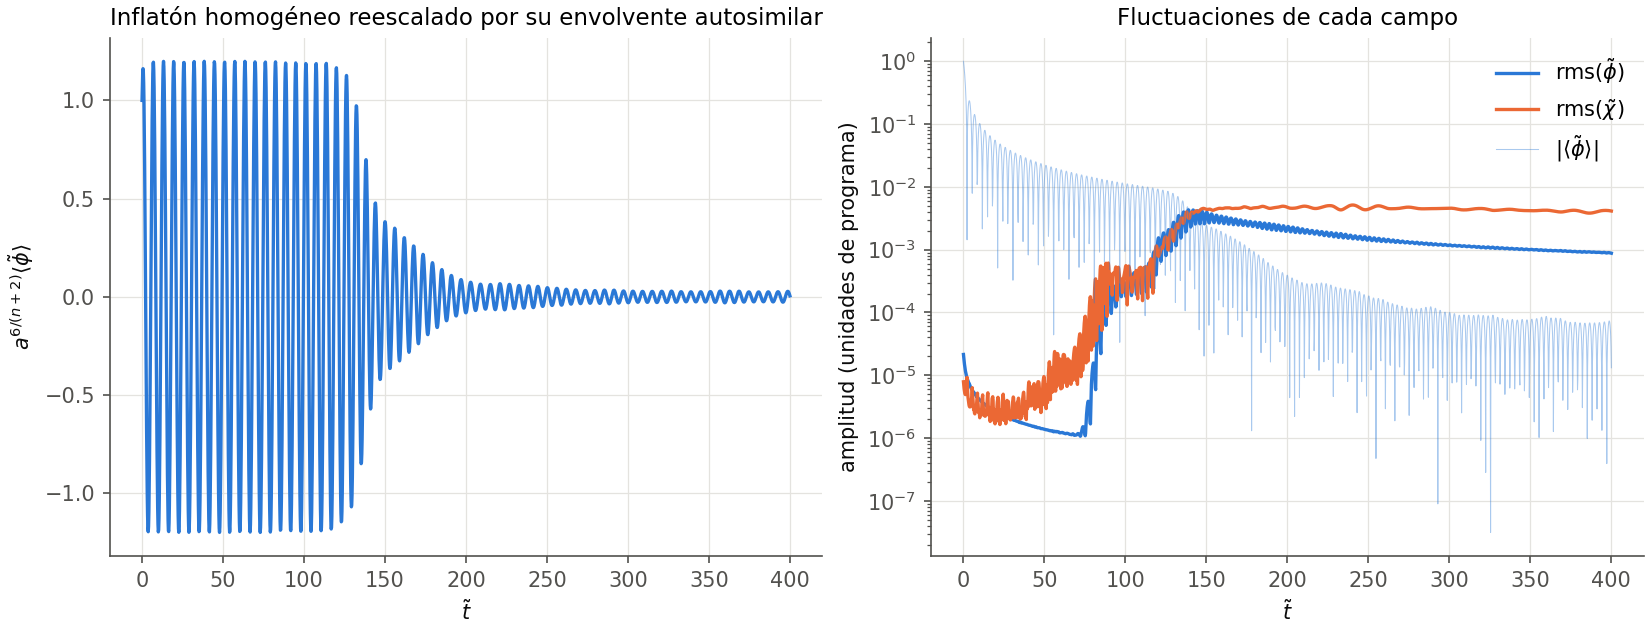
\includegraphics[width=\textwidth]{figuras/genmonomial_cuadratico_N64_campos.png}
                \caption{Monomial cuadrático de control ($m^2\phi^2/2$), $N = 64$. Izquierda: $\langle\tilde\phi\rangle$ multiplicado por $a^{6/(n+2)} = a^{3/2}$, que sin resonancia oscilaría con amplitud constante. Derecha: rms de cada campo y $|\langle\tilde\phi\rangle|$.}
                \label{fig:genmonomial_cuadratico-campos}
            \end{figure}
            \begin{figure}[H]
                \centering
                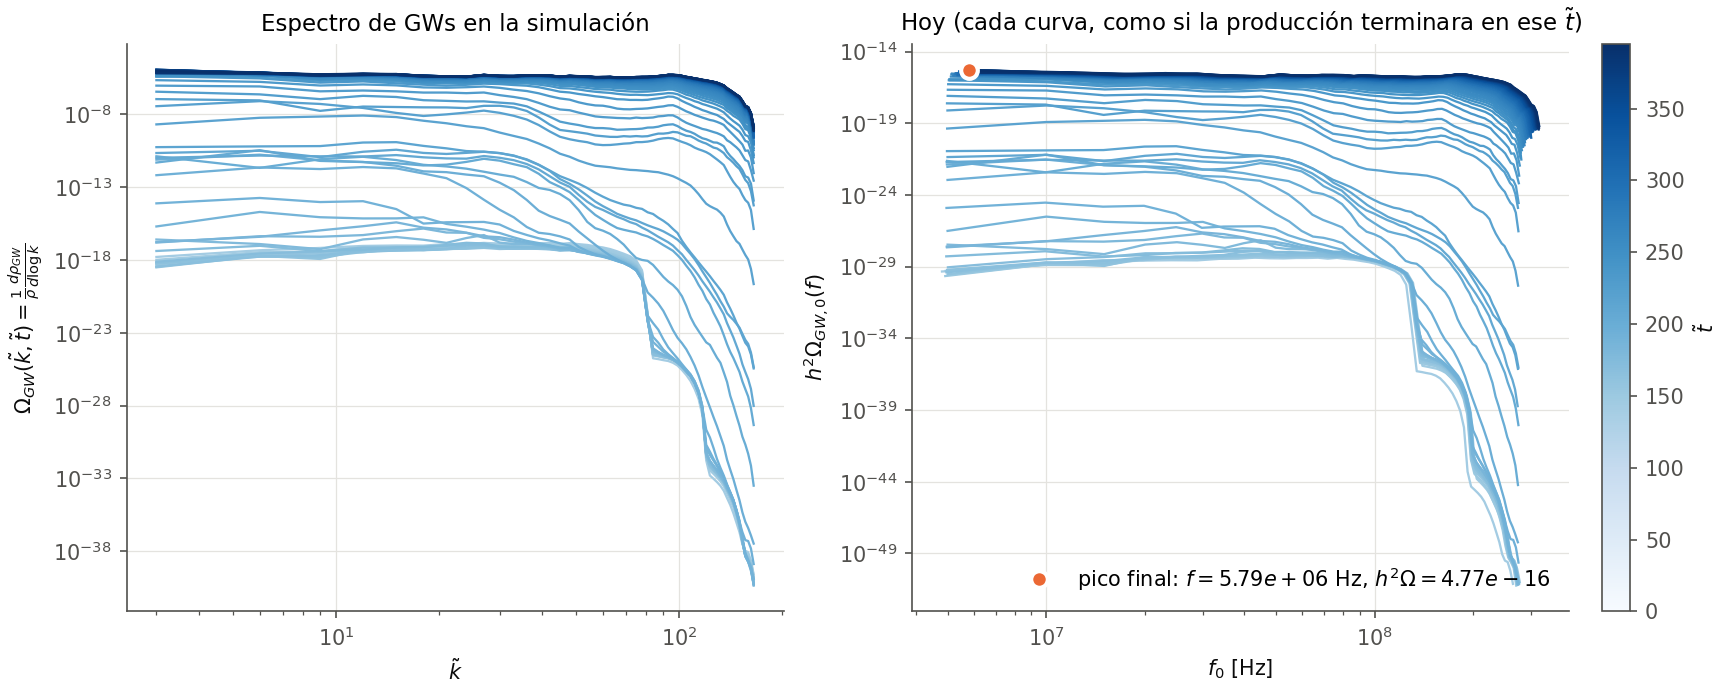
\includegraphics[width=\textwidth]{figuras/genmonomial_cuadratico_N64_gws.png}
                \caption{Monomial cuadrático de control ($m^2\phi^2/2$), $N = 64$. Espectro de GWs en la red (izquierda) y llevado a hoy con $T_{\text{RH}} = 10^{10}$\,GeV y $w = 0$ hasta el reheating (derecha), a cada tiempo de salida (claro = temprano).}
                \label{fig:genmonomial_cuadratico-gws}
            \end{figure}

            \texttt{genmonomial\_cuadratico.in} es $V = m^2\phi^2/2$ con la masa del T-model cuadrático ($\alpha_K = 1$), así que cerca del mínimo tiene el mismo potencial de programa. Está excluido por $r$ ($r = 0.15$ con $N_* = 51.8$). Arranca en $\phi_0 = \sqrt 2\,m_p$, con $a^{3/2}\langle\tilde\phi\rangle$ oscilando con amplitud $\simeq 1.2$, contra $1.09$ en el T-model (Fig.~\ref{fig:genmonomial_cuadratico-campos}).

            Al revés que en el caso cuártico (Sec.~\ref{sec:monomial-N64}), el monomial es el último en resonar: las GWs empiezan a crecer en $\tilde t \simeq 120$, contra $70$--$75$ en los $\alpha$-attractors, y la amplitud del condensado cae a la mitad en $\tilde t \simeq 140$ (T-model: 108). Aun así, es el que más GWs produce: $\rho_{GW}/\rho = 2.46 \times 10^{-5}$, el doble que el T-model, y el más saturado (crece un $4\%$ en los últimos 100 de $\tilde t$). Además tiene más potencia en el IR: $\Omega_{GW,e} \simeq 0.9 \times 10^{-5}$ en $\tilde k = 3$, contra $1.4 \times 10^{-6}$ en el T-model. Como todas las corridas parten de la misma realización de las fluctuaciones, la diferencia viene del potencial; lo que no sabemos, con una sola semilla, es cuánto cambiaría con otra realización.

            Hoy, con $T_{\text{RH}} = 10^{10}$\,GeV y $w = 0$, el máximo es $h^2\Omega_{GW,0} = 4.8 \times 10^{-16}$ en el primer bin ($5.8 \times 10^6$\,Hz), y más de la mitad del máximo cae hasta $1.9 \times 10^8$\,Hz (Fig.~\ref{fig:genmonomial_cuadratico-gws}). Con $\epsilon = 1$ daría $1.5 \times 10^{-10}$ en $1.4 \times 10^8$\,Hz.
}{}
    \IfFileExists{modelos/tmodel.tex}{    \section{T-models: $V = A\tanh^n(\phi/M)$}
        \label{sec:tmodel}

        Implementado en \texttt{models/gentmodel.h}; los \texttt{.in} son \texttt{gentmodel.in} ($n = 2.5$, exploratorio) y \texttt{gentmodel\_cuartico.in} (caso del paper, Sec.~\ref{sec:parametros-cuarticos}).
            
        \subsection{Derivadas}

            Consideremos que los potenciales de tipo T-model generales son de la forma
            \begin{equation}
                V(\phi) = A \tanh^n \left( \frac{\phi}{M} \right)
            \end{equation}

            Para la implementación de estos modelos en \CosmoLattice debemos calcular sus derivadas primera y segunda:
            \begin{equation}
                V^\prime (\phi) = \frac{A n}{M} \tanh^{n - 1} \left( \frac{\phi}{M} \right) \sech^2 \left( \frac{\phi}{M} \right)
            \end{equation}
            \begin{equation}
                V^{\prime \prime} (\phi) = \frac{A n}{M^2} \sech^2 \left( \frac{\phi}{M} \right) \tanh^{n - 2} \left( \frac{\phi}{M} \right) \left[ (n - 1) \sech^2 \left( \frac{\phi}{M} \right) - 2 \tanh^2 \left( \frac{\phi}{M} \right) \right]
            \end{equation}

        \subsection{Variables computacionales}

            El potencial de los T-models está acotado: satura en $A$ para $|\phi| \gg M$. Si eligiéramos $\omega_*$ pidiendo que el coeficiente de $\tanh^n(\tilde\phi/\tilde M)$ en $\tilde V$ sea exactamente $1$, $\omega_*$ no quedaría atado a la frecuencia física de oscilación alrededor de $\phi = 0$ y el $\alpha$ de la Sec.~\ref{sec:alpha} dejaría de cumplir su propósito. Seguimos en cambio el criterio de la Sec.~\ref{sec:variables}: durante el reheating el campo oscila en $|\phi| \ll M$, donde
            \begin{equation}
                V(\phi) = A \tanh^n \left( \frac{\phi}{M} \right) \underset{|\phi| \ll M}{\simeq} \frac{A}{M^n} \, |\phi|^n \, ,
            \end{equation}
            así que $A_{\text{eff}} = A/M^n$ y
            \begin{equation}
                \omega_*^2 = A_{\text{eff}} \, n \, \phi_0^{n - 2} = \frac{A n}{M^n} \, \phi_0^{n-2}
                \hspace{1cm} \Longrightarrow \hspace{1cm}
                \begin{cases}
                    \omega_* = \sqrt{A n} \, M^{-n/2} \, \phi_0^{n/2 - 1} \\
                    \displaystyle q = \frac{g^2 \phi_0^2}{\omega_*^2} = \frac{g^2 \phi_0^{4-n} M^n}{n A}
                \end{cases}
            \end{equation}
            Con esta elección, y definiendo nuevamente $\tilde{M} \equiv M/\phi_0$, el potencial de programa resulta (puede verificarse por sustitución directa de $\phi = \phi_0 \tilde\phi$, $\chi = \phi_0\tilde\chi$)
            \begin{equation}
                \tilde{V} \left( \tilde{\phi}, \tilde{\chi} \right) = \frac{1}{n} \left| \tilde{M} \tanh \left( \frac{\tilde{\phi}}{\tilde{M}} \right) \right|^n + \frac{1}{2} \, q \, \tilde{\phi}^2 \tilde{\chi}^2 \, ,
            \end{equation}
            que se reduce correctamente al caso monomial ($|\tilde\phi|^n/n$) en el límite $\tilde M \to \infty$ ($M \to \infty$ a $\phi_0$ fijo), y a \texttt{tanh2.h} para $n=2$ ($\omega_* = \sqrt{2A}/M \to \sqrt{\Lambda^4}/M$ con $A = \Lambda^4/2$), como debe ser.

        \subsection{Condiciones iniciales}

            La condición $\epsilon_V = 1$ (Sec.~\ref{sec:ci}) para este potencial:
            \begin{equation*}
                \begin{split}
                    \epsilon &= \frac{m_p^2}{2} \left[ \frac{V^\prime (\phi)}{V(\phi)} \right]^2\\
                    \frac{V^\prime (\phi)}{V(\phi)} &= \frac{n}{M} \frac{\sech^2 (\phi/M)}{\tanh (\phi/M)} = \frac{n}{M} \frac{1}{\sinh (\phi/M) \cosh (\phi/M)} = \frac{2n}{M} \csch \left( \frac{2\phi}{M} \right)\\
                    1 &= \frac{m_p^2}{2} \left[ \frac{2n}{M} \csch \left( \frac{2\phi_0}{M} \right) \right]^2\\
                    \frac{M^2}{2 n^2 m_p^2} &= \csch^2 \left( \frac{2 \phi_0}{M} \right)\\
                    \sinh \left( \frac{2 \phi_0}{M} \right) &= \frac{\sqrt{2} \, n \, m_p}{M}
                \end{split}
            \end{equation*}
            \begin{equation}
                \phi_0 = \frac{M}{2} \operatorname{arcsinh} \left( \frac{\sqrt{2} \, n \, m_p}{M} \right)
            \end{equation}

        \subsection{Momento inicial}
            \label{sec:momento-inicial-T}

            Por el argumento de la Sec.~\ref{sec:momento-inicial}, $\dot{\phi}_0 = -\sqrt{(\sqrt{7/3} - 1) \, A \tanh^n(\phi_0/M)}$. Con los parámetros de \texttt{gentmodel.in} ($n = 2.5$, $M = 10\,m_p$) da $\dot\phi_0 = -1.914 \times 10^{31}\,\text{GeV}^2$. El final exacto de la inflación ($\epsilon_H = 1$) cae en $\phi = 3.18 \times 10^{18}\,\text{GeV}$, contra $\phi_0 = 4.22 \times 10^{18}\,\text{GeV}$.}{}
    \IfFileExists{modelos/emodel.tex}{    \section{E-models: $V = A(1 - e^{-\phi/M})^n$}
        \label{sec:emodel}

        Implementado en \texttt{models/genemodel.h}; los \texttt{.in} son \texttt{genemodel.in} ($n = 2.5$, exploratorio), \texttt{genemodel\_cuartico.in} y \texttt{genemodel\_cuartico\_aK5.in} (casos del paper, Sec.~\ref{sec:parametros-cuarticos}).

        \subsection{Derivadas}

            Consideremos que los potenciales de tipo E-model generales son de la forma
            \begin{equation}
                V(\phi) = A \left( 1 - e^{-\phi/M} \right)^n
            \end{equation}

            Para la implementación de estos modelos en \CosmoLattice debemos calcular sus derivadas primera y segunda. Definiendo $u \equiv 1 - e^{-\phi/M}$ (de modo que $1 - u = e^{-\phi/M}$ y $u^\prime = (1-u)/M$), tenemos
            \begin{equation*}
                \begin{split}
                    V^\prime (\phi) &= A n \, u^{n-1} \, u^\prime = \frac{An}{M} \, u^{n-1} (1-u)
                \end{split}
            \end{equation*}
            \begin{equation}
                V^\prime (\phi) = \frac{A n}{M} \left( 1 - e^{-\phi/M} \right)^{n-1} e^{-\phi/M}
            \end{equation}
            y derivando nuevamente
            \begin{equation*}
                \begin{split}
                    \frac{d}{d\phi} \left[ u^{n-1} (1-u) \right] &= u^\prime \, u^{n-2} \left[ (n-1)(1-u) - u \right] = u^\prime \, u^{n-2} \left[ (n-1) - n u \right]\\
                    V^{\prime\prime} (\phi) &= \frac{An}{M^2} \, u^{n-2} (1-u) \left[ (n-1) - n u \right]
                \end{split}
            \end{equation*}
            \begin{equation}
                V^{\prime \prime} (\phi) = \frac{A n}{M^2} \, e^{-\phi/M} \left( 1 - e^{-\phi/M} \right)^{n-2} \left[ n \, e^{-\phi/M} - 1 \right]
            \end{equation}

        \subsection{Variables computacionales}

            El potencial de los E-models está acotado por un lado: satura en $A$ para $\phi \gg M$ (aunque no del lado $\phi \ll -M$, donde crece exponencialmente, lo que vuelve asimétricas las oscilaciones posteriores; para $n$ no entero, en $\phi<0$ usamos $|1 - e^{-\phi/M}|^n$, igual que el código). Con el criterio de la Sec.~\ref{sec:variables}, $\omega_*$ y $q$ salen del comportamiento local cerca de $\phi = 0$, la región relevante durante el reheating, y no de la altura global $A$:
            \begin{equation}
                V(\phi) = A \left( 1 - e^{-\phi/M} \right)^n \underset{|\phi| \ll M}{\simeq} \frac{A}{M^n} \, |\phi|^n \, ,
            \end{equation}
            de modo que $A_{\text{eff}} = A/M^n$ y
            \begin{equation}
                \omega_*^2 = A_{\text{eff}} \, n \, \phi_0^{n-2} = \frac{A n}{M^n} \, \phi_0^{n-2}
                \hspace{1cm} \Longrightarrow \hspace{1cm}
                \begin{cases}
                    \omega_* = \sqrt{A n} \, M^{-n/2} \, \phi_0^{n/2 - 1} \\
                    \displaystyle q = \frac{g^2 \phi_0^2}{\omega_*^2} = \frac{g^2 \phi_0^{4-n} M^n}{n A}
                \end{cases}
            \end{equation}
            Son los mismos $\omega_*$ y $q$ que en los T-models, porque ambos potenciales tienen el mismo comportamiento cerca de $\phi = 0$. Definiendo nuevamente $\tilde{M} \equiv M/\phi_0$, el potencial de programa resulta
            \begin{equation}
                \tilde{V} \left( \tilde{\phi}, \tilde{\chi} \right) = \frac{1}{n} \left| \tilde{M} \left( 1 - e^{-\tilde{\phi}/\tilde{M}} \right) \right|^n + \frac{1}{2} \, q \, \tilde{\phi}^2 \tilde{\chi}^2 \, ,
            \end{equation}
            que también se reduce correctamente al caso monomial en el límite $\tilde M \to \infty$.

        \subsection{Condiciones iniciales}

            La condición $\epsilon_V = 1$ (Sec.~\ref{sec:ci}) para este potencial:
            \begin{equation*}
                \begin{split}
                    \epsilon &= \frac{m_p^2}{2} \left[ \frac{V^\prime (\phi)}{V(\phi)} \right]^2\\
                    \frac{V^\prime (\phi)}{V(\phi)} &= \frac{n}{M} \frac{1-u}{u} = \frac{n}{M} \frac{e^{-\phi/M}}{1 - e^{-\phi/M}} = \frac{n}{M} \frac{1}{e^{\phi/M} - 1}\\
                    1 &= \frac{m_p^2}{2} \left[ \frac{n}{M} \frac{1}{e^{\phi_0/M} - 1} \right]^2\\
                    \left( e^{\phi_0/M} - 1 \right)^2 &= \frac{n^2 m_p^2}{2 M^2}\\
                    e^{\phi_0/M} &= 1 + \frac{n \, m_p}{\sqrt{2} \, M}
                \end{split}
            \end{equation*}
            \begin{equation}
                \phi_0 = M \ln \left( 1 + \frac{\sqrt{2}}{2} \frac{n \, m_p}{M} \right)
            \end{equation}

        \subsection{Momento inicial}
            \label{sec:momento-inicial-E}

            Por el argumento de la Sec.~\ref{sec:momento-inicial}, $\dot{\phi}_0 = -\sqrt{(\sqrt{7/3} - 1) \, A \left(1 - e^{-\phi_0/M}\right)^n}$. Con los parámetros de \texttt{genemodel.in} ($n = 2.5$, $M = 10\,m_p$) da $\dot\phi_0 = -1.621 \times 10^{31}\,\text{GeV}^2$. El final exacto de la inflación ($\epsilon_H = 1$) cae en $\phi = 2.95 \times 10^{18}\,\text{GeV}$, contra $\phi_0 = 3.96 \times 10^{18}\,\text{GeV}$.}{}

\end{document}
